\documentclass[electronics,article,submit,pdftex,moreauthors]{Definitions/mdpi}

\usepackage{pgfplots}
\usepgfplotslibrary{groupplots}
\pgfplotsset{compat=1.18}
\usetikzlibrary{arrows.meta,calc,fit,positioning}

\definecolor{slowcolor}{RGB}{45,112,180}
\definecolor{mediumcolor}{RGB}{230,126,34}
\definecolor{fastcolor}{RGB}{35,139,69}

\firstpage{1}
\pubvolume{1}
\issuenum{1}
\articlenumber{0}
\pubyear{2026}
\copyrightyear{2026}
\datereceived{ }
\daterevised{ }
\dateaccepted{ }
\datepublished{ }
\setlength{\headheight}{20pt}

\newcommand{\etal}{et~al.}
\newcommand{\mobile}{MobileNetV2}
\newcommand{\resnet}{ResNet-50}
\newcommand{\jetson}{NVIDIA Jetson Orin Nano}
\newcommand{\imagenet}{ImageNet}
\newcommand{\fwd}{\mathrm{fwd}}
\newcommand{\logwin}{\mathrm{log}}
\providecommand{\figref}[1]{Figure~\ref{#1}}
\renewcommand{\tabref}[1]{Table~\ref{#1}}
% Generated by analysis/build_revision_results.py; do not edit manually.
\newcommand{\TotalRuns}{558}
\newcommand{\PrimaryRuns}{378}
\newcommand{\PrimaryConfigurations}{126}
\newcommand{\PrimaryDevices}{3}
\newcommand{\TotalEvaluatedImagesMillions}{27.9}
\newcommand{\MobileFpThirtyTwoThroughputRatio}{0.694}
\newcommand{\ResnetFpThirtyTwoThroughputRatio}{0.519}
\newcommand{\MobileFpThirtyTwoEnergyRatio}{1.196}
\newcommand{\ResnetFpThirtyTwoEnergyRatio}{1.625}
\newcommand{\MobileFpSixtyFourThroughputRatio}{0.136}
\newcommand{\ResnetFpSixtyFourThroughputRatio}{0.0330}
\newcommand{\MobileFpSixtyFourEnergyRatio}{2.996}
\newcommand{\ResnetFpSixtyFourEnergyRatio}{12.41}
\newcommand{\SlowThroughputCv}{0.057}
\newcommand{\MediumThroughputCv}{0.500}
\newcommand{\FastThroughputCv}{28.69}
\newcommand{\FastEnergyCv}{14.86}
\newcommand{\MaximumObservedTemperature}{53.7}
\newcommand{\RunsWithLargeStalls}{15}
\newcommand{\LargeStallIterations}{28}
\newcommand{\MaximumStallSensitivity}{16.64}

% Generated by analysis/long_run_drift_analysis.py; do not edit manually.
% Descriptive existing-data diagnostics only; no causal or population inference.
\newcommand{\PrimaryDurationUpperQuartileSeconds}{3885.75}
\newcommand{\PrimaryDurationUpperQuartileHours}{1.079}
\newcommand{\PrimaryAdjacentTransitionCount}{375}
\newcommand{\PrimaryStateEventGapMedianMilliseconds}{0.920}
\newcommand{\PrimaryStateEventGapPninetyfiveMilliseconds}{5.757}
\newcommand{\PrimaryStateEventGapMaximumMilliseconds}{91.624}
\newcommand{\FpSixtyFourSuccessorForwardRatio}{1.0024}
\newcommand{\FpSixtyFourSuccessorForwardRatioLoboMinimum}{1.0012}
\newcommand{\FpSixtyFourSuccessorForwardRatioLoboMaximum}{1.0052}
\newcommand{\FpSixtyFourSuccessorEnergyRatio}{0.9992}
\newcommand{\FpSixtyFourSuccessorEnergyRatioLoboMinimum}{0.9981}
\newcommand{\FpSixtyFourSuccessorEnergyRatioLoboMaximum}{1.0007}
\newcommand{\FpSixtyFourSuccessorStartTemperatureDeltaC}{-0.823}
\newcommand{\FpSixtyFourSuccessorStartTemperatureDeltaCLoboMinimum}{-1.001}
\newcommand{\FpSixtyFourSuccessorStartTemperatureDeltaCLoboMaximum}{-0.678}
\newcommand{\FpSixtyFourSuccessorExposedCount}{70}
\newcommand{\FpSixtyFourSuccessorReferenceCount}{179}
\newcommand{\LongPredecessorSuccessorForwardRatio}{1.0008}
\newcommand{\LongPredecessorSuccessorForwardRatioLoboMinimum}{0.9990}
\newcommand{\LongPredecessorSuccessorForwardRatioLoboMaximum}{1.0033}
\newcommand{\LongPredecessorSuccessorEnergyRatio}{1.0010}
\newcommand{\LongPredecessorSuccessorEnergyRatioLoboMinimum}{0.9993}
\newcommand{\LongPredecessorSuccessorEnergyRatioLoboMaximum}{1.0037}
\newcommand{\LongPredecessorSuccessorStartTemperatureDeltaC}{-1.235}
\newcommand{\LongPredecessorSuccessorStartTemperatureDeltaCLoboMinimum}{-1.287}
\newcommand{\LongPredecessorSuccessorStartTemperatureDeltaCLoboMaximum}{-1.185}
\newcommand{\LongPredecessorSuccessorExposedCount}{52}
\newcommand{\LongPredecessorSuccessorReferenceCount}{197}
\newcommand{\PrimaryForwardDriftEndStartRatio}{0.9973}
\newcommand{\PrimaryForwardDriftEndStartRatioLoboMinimum}{0.9952}
\newcommand{\PrimaryForwardDriftEndStartRatioLoboMaximum}{0.9995}
\newcommand{\PrimaryEnergyDriftEndStartRatio}{0.9921}
\newcommand{\PrimaryEnergyDriftEndStartRatioLoboMinimum}{0.9891}
\newcommand{\PrimaryEnergyDriftEndStartRatioLoboMaximum}{0.9953}
\newcommand{\PrimaryStartTemperatureDriftEndStartDeltaC}{0.363}
\newcommand{\PrimaryStartTemperatureDriftEndStartDeltaCLoboMinimum}{-0.129}
\newcommand{\PrimaryStartTemperatureDriftEndStartDeltaCLoboMaximum}{0.692}
\newcommand{\HistoricalRandomForwardPositionRho}{-0.353}
\newcommand{\HistoricalRandomEnergyPositionRho}{0.298}


\Title{Measurement Boundaries and Sequence-Dependent Hardware-State Realization in Edge-AI Energy Benchmarking: A Blocked Factorial Study on the NVIDIA Jetson Orin Nano}

\newcommand{\orcidauthorA}{0009-0005-0328-4664}
\newcommand{\orcidauthorB}{0000-0001-8217-7149}
\newcommand{\orcidauthorC}{0000-0001-6658-0288}

\Author{Adem Tek $^{1,2}$, Lucas Wei{\ss}beck $^{1,}$*\orcidA{}, Alexander Rachmann $^{1}$\orcidB{} and Hendrik Poschmann $^{1}$\orcidC{}}
\AuthorNames{Adem Tek, Lucas Wei{\ss}beck, Alexander Rachmann and Hendrik Poschmann}

\address{%
$^{1}$ \quad Hochschule Niederrhein University of Applied Sciences, Reinarzstra{\ss}e 49, 47805 Krefeld, Germany; adem.tek@stud.hn.de (A.T.); lucas.weissbeck@hs-niederrhein.de (L.W.); alexander.rachmann@hs-niederrhein.de (A.R.); hendrik.poschmann@hs-niederrhein.de (H.P.); \\
$^{2}$ \quad Current affiliation: Independent Researcher, Staufenberg, Germany}

\corres{Correspondence: lucas.weissbeck@hs-niederrhein.de}

\abstract{Edge artificial-intelligence (AI) inference energy comparisons can mislead when timing, system-energy integration, and requested hardware states are conflated. We audited 558 Jetson Orin Nano runs; the balanced primary design comprised 378 runs on three distinct physical boards, spanning two convolutional neural networks (CNNs), FP16/FP32/FP64 tensor dtypes, seven batch sizes, and three requested profile branches. Forward performance was separated from onboard input-rail (\texttt{VDD\_IN}) energy over the logged window. In the full grid, precision accounted for 71.5\% of log-scale forward-throughput variation and 66.4\% of logged-window energy variation, largely reflecting FP64 stress. In the FP16/FP32 slow+medium sensitivity, batch instead accounted for 54.1\% of forward-throughput variation. Across these cross-board-stable branches, FP32 retained 68.4\% and 54.8\% of FP16 throughput for \mobile{} and \resnet{}, while using 1.212 and 1.612 times the logged energy. At batch one, FP16 retained only 85.4\% and 84.7\% of FP32 throughput. All 126 requested-fast runs exhibited an exact observed association: the realized low/high clock regime matched whether the last non-fast predecessor was slow (57/57) or medium (69/69). Thus, requested profile labels did not define independently realized treatments. Reliable claims require compatible measurement boundaries, explicit protocol overheads, and verified state reset/read-back.}

\keyword{edge AI; energy measurement; embedded GPU; Jetson Orin Nano; numerical precision; batch size; measurement boundary; hardware-state fidelity; state realization; reproducibility}

\begin{document}

\section{Introduction}

Image analysis is increasingly moved from remote data centers to devices located near cameras and sensors. This placement can reduce network dependence and response time and can keep raw visual data local, but it transfers compute, power, and thermal constraints to the deployed device \cite{koubaa2022cloud,rey2025drone}. Energy is therefore an engineering constraint alongside accuracy and latency. Green-artificial-intelligence (AI) reviews and algorithm-level energy-efficiency studies emphasize that meaningful efficiency assessment must connect algorithmic choices to measured resource consumption rather than treating model accuracy as the only objective \cite{bolon2024green,penev2024energy}.

An inference configuration is more than a neural-network architecture. Numerical precision, batch formation, runtime, host-side preprocessing, memory traffic, and power management jointly determine useful work per joule \cite{yang2017method,hodak2021recent}. Embedded graphics-processing-unit (GPU) studies likewise show that rankings can change with the device and software path \cite{jo2020benchmarking,suzen2020benchmark}. A low average power value is not sufficient evidence of low energy per inference: if a low-clock configuration takes proportionally longer, its total energy can be higher.

Measurement boundaries create an additional risk. A synchronized model-forward timer can describe accelerator-facing computation, whereas a board-power trace may also contain Python startup, model loading, warm-up, data transformations, accuracy calculation, and logger overhead. Dividing the latter energy by the former time silently combines incompatible quantities. Standardized efforts such as MLPerf make scenario and timing rules explicit for this reason \cite{reddi2020mlperf,banbury2021mlperf}. Board-level energy studies require the same discipline.

This study evaluates two convolutional neural networks (CNNs), three floating-point formats, seven batch sizes, and three requested power-profile branches on a \jetson{}. Its central objective is methodological as well as empirical: every archived performance and power file is reprocessed, forward-only and logged-window quantities are kept separate, and requested profile labels are checked against realized clock traces. That state check reveals an exact observed association between the requested fast branch's realized clock regime and its most recent non-fast predecessor, turning a nominal configuration factor into a direct example of why randomized order cannot substitute for treatment verification.

The main research question is: \emph{How do model, requested tensor dtype, batch size, and requested power-profile selection affect forward performance and logged-window energy for CNN classification on the tested Jetson Orin Nano setup?} We address three subordinate questions:
\begin{itemize}
    \item \textbf{RQ1:} Which factors and interactions account for the observed variation in forward throughput, logged-window throughput, input power, and logged-window energy per evaluated image, and how do conclusions change when the FP64 stress level is excluded?
    \item \textbf{RQ2:} How do precision and batch size interact across three physical-board blocks, including batch-one forward execution?
    \item \textbf{RQ3:} Do requested power-profile branches produce independently realized states, or are their realized regimes associated with the preceding branch?
\end{itemize}

The contributions are:
\begin{itemize}
    \item a balanced $3\times2\times3\times7\times3$ device-by-configuration data set with one complete run per cell and \PrimaryRuns{} primary runs;
    \item an auditable distinction between synchronized forward performance and integrated input energy over the logged window, including batch-dependent benchmark overhead;
    \item physical-board-blocked contrasts, a complete factorial decomposition, and FP16/FP32 and no-fast sensitivity analyses, without treating batches or timestamped power samples as independent units;
    \item a transition analysis showing an exact 126/126 observed association between the realized requested-fast clock regime and the most recent slow or medium branch;
    \item a reusable reporting checklist for measurement-boundary alignment, state reset/read-back, code identity, replication, and power metrology; and
    \item an integrity audit covering all \TotalRuns{} archived runs, \TotalEvaluatedImagesMillions{} million evaluated images, per-batch records, raw logs, parsed power traces, manifests, and analysis inputs.
\end{itemize}

\section{Related Work}

\subsection{Energy-Aware Edge Inference}

Direct measurement on the target platform is necessary because operation counts alone do not capture data movement, memory-system behavior, runtime overhead, or board power \cite{yang2017method}. Comparative vision studies consequently evaluate model choice under device-specific constraints \cite{mira2024benchmarking}. Cross-device benchmarks have reported substantial differences among GPU-accelerated edge platforms \cite{jo2020benchmarking,suzen2020benchmark}, while cloud-versus-edge studies show that the relevant system boundary depends on the deployment scenario \cite{koubaa2022cloud}. These results motivate a within-platform factorial experiment rather than a universal device ranking.

\mobile{} uses inverted residuals and linear bottlenecks to reduce computation for resource-constrained applications \cite{sandler2018mobilenetv2}. \resnet{} provides a heavier residual-network reference with higher standard ImageNet accuracy \cite{he2016deep}. Their comparison represents a lightweight-versus-accuracy-oriented CNN contrast; it does not represent transformers, detectors, or segmentation networks. For example, camera-based object-detection pipelines have different preprocessing and latency requirements \cite{rey2025drone}.

\subsection{Precision, Runtime, Batching, and Power Management}

Reduced precision can improve throughput when the accelerator and runtime expose an appropriate execution path. Conversely, double precision may be disproportionately expensive on embedded accelerators. Runtime choice is inseparable from that conclusion: TensorRT applies graph and kernel optimizations that can change latency, memory use, and precision behavior relative to eager PyTorch \cite{jeong2022tensorrt,nvidiatensorrt}. Recent Orin Nano work already evaluates batch size, precision, TensorRT, and energy for a transformer workload \cite{martinsalinas2025}, while application studies cover multiple You Only Look Once (YOLO) models, arithmetic formats, and nominal power modes \cite{rey2025drone,mela2025yolo}. The present experiment intentionally measures direct PyTorch execution; TensorRT is outside its experimental scope, as are automatic mixed precision, 8-bit integer (INT8) execution, and compiler-generated engines.

Batching can amortize launch and host overhead and increase throughput, but it also changes forward duration and may be infeasible for a request stream. Benchmark suites distinguish offline, server, and single-stream scenarios for this reason \cite{reddi2020mlperf,banbury2021mlperf}. The batch-size-one measurements here describe forward-only duration for one already-prepared batch under the reference-code timing interpretation; they do not include queueing or camera-to-result latency.

Frequency selection can alter performance and energy nonlinearly. Work on integrated central-processing-unit (CPU)--GPU governors demonstrates interactions among workload phase, CPU clocks, GPU clocks, and memory behavior \cite{karzhaubayeva2023cnn}. A profile name is therefore not an experimental treatment unless its realized state is verified. We report requested settings and observed telemetry separately and refrain from equating three shell-script labels with three idealized fixed dynamic-voltage-and-frequency-scaling (DVFS) points.

Recent studies illustrate complementary measurement scopes. Martin-Salinas \etal{} compare batch, precision, compilation, memory, and energy on one Orin Nano using internal sensors \cite{martinsalinas2025}. Aramendia \etal{} measure full-process energy for YOLOv5n across three embedded platforms \cite{aramendia2025}. Giedra \etal{} combine internal Jetson telemetry with an external input measurement for large-language-model (LLM) inference \cite{giedra2026}. \tabref{tab:related-comparison} positions these measurement boundaries and blocking choices against the present study. The cited work raises the benchmark breadth and metrology baseline; it does not, however, make requested clock-state fidelity and sequence-dependent state realization its experimental object.

\begin{table*}[t]
\caption{Positioning against recent deployment-oriented edge-inference studies. ``Not reported'' means that the cited study does not make independent hardware blocks or requested-versus-realized clock-state verification a principal reported design element. SSAST: self-supervised audio spectrogram transformer; LLM: large language model; CNN: convolutional neural network; CPU/GPU: central/graphics processing unit; INT8: 8-bit integer; FP16/FP32/FP64: requested 16-/32-/64-bit floating-point tensor dtype; \texttt{VDD\_IN}: onboard input-power rail.}
\label{tab:related-comparison}
\centering
\small
\setlength{\tabcolsep}{2pt}
\begin{tabularx}{\textwidth}{>{\raggedright\arraybackslash}p{22mm}>{\raggedright\arraybackslash}p{27mm}>{\raggedright\arraybackslash}p{30mm}>{\raggedright\arraybackslash}X>{\raggedright\arraybackslash}p{36mm}}
\toprule
Study & Workload/runtime & Configuration scope & Energy boundary/source & Replication/state verification \\
\midrule
Martin-Salinas \etal{} \cite{martinsalinas2025} & SSAST; PyTorch/TensorRT & Batch, FP32/FP16/INT8, CPU/GPU & Inference-cycle energy; 10 Hz internal sensors & One Orin Nano; independent blocks and state read-back not reported \\
Aramendia \etal{} \cite{aramendia2025} & YOLOv5n; platform runtimes & Three embedded platforms & Full inference-process energy & Platform comparison; state read-back not reported \\
Giedra \etal{} \cite{giedra2026} & 12 LLMs; Ollama & Model size, CPU/GPU & Generation session; internal telemetry plus external input measurement & Independent blocks and state read-back not reported \\
This study & Two CNNs; eager PyTorch & FP16/FP32/FP64, batch 1--128, requested profiles & First-to-last logged \texttt{VDD\_IN} samples & Three distinct physical boards; trace-level state and sequence transitions audited \\
\bottomrule
\end{tabularx}
\end{table*}

\subsection{Research Gap}

The present contribution is therefore not another claim that half precision or batching can improve a Jetson benchmark. It is a matched factorial analysis that keeps forward and logged-window estimands separate, treats the physical board rather than the batch or power sample as the blocking unit, and tests whether a requested power branch is independently realized. This last check is essential: without it, a statistically precise comparison can still estimate an ill-defined or path-associated treatment.

\section{Materials and Methods}

\subsection{Hardware, Software, and Archived Identity}

The experiments were conducted on three physically distinct Jetson Orin Nano Developer Kits, author-confirmed as the devices represented by \texttt{Clone1--3}. All raw \texttt{tegrastats} records report 7620 MB usable memory, consistent with the 8 GB developer-kit variant. The Jetson Orin Nano combines CPU, GPU, and unified memory for embedded AI workloads \cite{nvidiajetson}. The per-run metadata record PyTorch 2.6.0, Torchvision 0.21.0, and \texttt{cuda\_device="Orin"}; NVIDIA Compute Unified Device Architecture (CUDA) details are not otherwise embedded. The supplied experiment documentation identifies JetPack 6.2, Linux for Tegra 36.4.3, and Ubuntu 22.04, but these values are not embedded in the per-run metadata and are therefore author-reported rather than artifact-verified. Inference ran in a Jetson-compatible container \cite{paszke2019pytorch,jetsoncontainers}; its image digest was not archived.

Module serial numbers and product IDs were not retained, so the author-confirmed board identities cannot be independently recovered from the artifacts. The laboratory was air-conditioned at a nominal ambient temperature of 24~$^\circ$C, held equal across the three boards; no time-resolved ambient-temperature record, external supply voltage/current record, or external power-analyzer measurement was archived. The three complete \texttt{Clone1--3} folders form the physical-board blocking factor, but board, seed, order, and temporal effects remain associated and a pure silicon-to-silicon variance component is not estimated. \texttt{MasterJetson} is excluded from primary inference because it contains only batch sizes 1--16 and its observed external-memory-controller (EMC) mode is 3199 MHz rather than 2133 MHz. It remains in the integrity audit.

The campaign roles and exclusions summarized in \tabref{tab:campaigns} were fixed before the primary factorial analysis described below.

\begin{table*}[t]
\caption{Archived campaigns and their inferential role. Each run evaluates all 50,000 validation images.}
\label{tab:campaigns}
\centering
\small
\resizebox{\linewidth}{!}{%
\begin{tabular}{lccccl}
\toprule
Campaign & Runs & Batches & Seed & EMC mode & Inferential role \\
\midrule
Ordered March reference & 54 & 32--128 & 123 & 2133 MHz & Descriptive historical comparison \\
Randomized March reference & 54 & 32--128 & 123 & 3199 MHz & Descriptive historical comparison \\
MasterJetson & 72 & 1--16 & 123 & 3199 MHz & Audit and scope check only \\
Clone1 & 126 & 1--128 & 42 & 2133 MHz & Primary device block \\
Clone2 & 126 & 1--128 & 789 & 2133 MHz & Primary device block \\
Clone3 & 126 & 1--128 & 456 & 2133 MHz & Primary device block \\
\bottomrule
\end{tabular}}
\end{table*}

\subsection{Models, Data, Preprocessing, and Floating-Point Semantics}

The archived metadata identify pretrained \mobile{} and \resnet{} models but do not store checkpoint hashes. They establish that each run evaluated the complete 2012 ImageNet validation set ($N=50{,}000$) and retained the final partial batch \cite{deng2009imagenet,russakovsky2015ilsvrc}. The inspected reference implementation requests \texttt{MobileNet\_V2\_Weights.DEFAULT} and \texttt{ResNet50\_Weights.DEFAULT}; under Torchvision 0.21.0 these resolve to the respective \texttt{IMAGENET1K\_V2} weights. It resizes the shorter dimension to 224 pixels using bilinear interpolation, center-crops to $224\times224$, converts to tensors, normalizes with the standard ImageNet channel means and standard deviations, and configures the loader with \texttt{shuffle=False}, \texttt{num\_workers=0}, pinned host memory, and \texttt{drop\_last=False}. Because the exact July executable is unavailable, the checkpoint mapping, preprocessing path, and loader settings are provenance-qualified reconstructions from the reference source rather than per-run artifact facts.

Per-run metadata label the requested tensor dtype as FP16, FP32, or FP64. In the inspected reference implementation, model parameters and input tensors are explicitly cast with \texttt{.to(dtype)}, inference uses \texttt{torch.no\_grad()} without automatic mixed precision or autocasting, TensorFloat-32 (TF32) is disabled, deterministic algorithms and deterministic cuDNN behavior are requested, and cuDNN benchmarking is disabled. Because the exact July executable is not linked by an archived Git commit, those backend flags are properties of the verified reference source rather than artifact-level per-run facts. No archived output identifies a TensorRT engine, quantization, fallback detector, or per-operator precision trace. Consequently, FP16, FP32, and FP64 denote requested PyTorch tensor dtypes, not a verified operator-level or TensorRT precision contract. Top-1 accuracy was recomputed as a control outcome.

\subsection{Primary Factorial Design and Randomization}

For each of the three primary physical boards, the complete grid contains
\begin{equation}
2\ \text{models}\times3\ \text{precisions}\times7\ \text{batch sizes}\times3\ \text{profiles}=126
\end{equation}
runs. The factors are model (\mobile{}, \resnet{}), precision (FP16, FP32, FP64), batch size (1, 4, 8, 16, 32, 64, 128), and nominal profile (slow, medium, fast). Each physical board used a different seed to create a Python pseudorandom permutation of all 126 configurations. The archived state events exactly match the manifest order; the three permutations contain 86, 94, and 84 profile transitions, respectively.

To test state independence, runs were ordered by the archived \texttt{running} events in each board folder's \texttt{grid\_state.jsonl}; this event order is monotonic and agrees with manifest and timestamp chronology. For every requested fast run, we recorded both the immediately preceding requested profile and the most recent preceding non-fast profile. The fast GPU regime was classified from the modal logged GPU frequency; the observed modes form two disjoint groups, 407 MHz and 812--815 MHz, so a classification cutoff at 600 MHz is unambiguous for these data. This transition analysis was specified after the bimodality was observed and is therefore diagnostic rather than a randomized causal contrast.

There is one run per physical-board--configuration cell. The seed is therefore perfectly associated with board and run order. The reference implementation fixes the pretrained evaluation model and image order with \texttt{shuffle=False}, making a direct data-order effect of the seed unlikely if that code path was executed; however, deterministic backend flags are not verified in the per-run artifacts, and seed, board, and temporal effects cannot be separated empirically. Batch iterations and power samples are repeated observations within a run, not experimental replicates.

\subsection{Requested Profiles and Realized State}

The inspected reference power-control script requests the states in \tabref{tab:profiles}. For slow and medium, it writes CPU, GPU, and EMC caps and stops the \texttt{nvpmodel} service; for fast, it invokes \texttt{jetson\_clocks --fan} when available. Because the exact July executable is unavailable, these commands document the intended control path rather than command-level proof for every run. The raw logs contain CPU frequencies, GPU activity and frequencies, EMC activity and frequencies, temperatures, and input-rail power, but no \texttt{nvpmodel} identifier, fan duty, explicit throttle flag, or supply voltage/current measured outside the module.

\begin{table*}[t]
\caption{Nominal profile commands and states observed on the three primary physical boards. Requested caps are not assumed to equal realized clocks.}
\label{tab:profiles}
\centering
\small
\begin{tabularx}{\textwidth}{l>{\raggedright\arraybackslash}X>{\raggedright\arraybackslash}X}
\toprule
Label & Requested action & Observed state in archived logs \\
\midrule
slow & CPU cap 729.6 MHz; GPU range 306--408 MHz; EMC cap 800 MHz & CPU mode 729 MHz; GPU modes 305 or 407 MHz with maximum 408 MHz; EMC mode 2133 MHz in every run \\
\addlinespace[3pt]
medium & CPU cap 1.2 GHz; GPU range 306--816 MHz; EMC cap 1600 MHz & CPU usually 1190 MHz; workload-varying GPU modes from 305 to approximately 815 MHz; EMC mode 2133 MHz in every run \\
\addlinespace[3pt]
fast & \texttt{jetson\_clocks --fan}, otherwise manually request maxima & Two inherited regimes: CPU/GPU approximately 729/407 MHz after the last slow branch (57/57) and 1190/812--815 MHz after the last medium branch (69/69); EMC mode 2133 MHz in every run \\
\bottomrule
\end{tabularx}
\end{table*}

The observed EMC state does not reproduce the requested 800/1600 MHz caps. More decisively, all 126 fast runs are perfectly associated with the preceding state: fast immediately after slow is low-clock in 42/42 cases, immediately after medium is high-clock in 41/41 cases, and fast after fast retains the prior low/high state in 43/43 cases. We therefore retain profile only as a factor describing the requested script branch. Its coefficients and interactions are descriptive and are not estimates of three clean, independently assigned clock treatments.

\subsection{Execution Workflow and Measurement Boundaries}

The inspected reference host workflow selects a nominal profile, starts \texttt{tegrastats} at a requested 1000 ms interval, waits 2 s, runs the Python benchmark, stops the logger, and moves the artifacts. Public repository commit \texttt{\seqsplit{1a66056ec3faf32a2fe56e10747932bf93aa856d}} was used for cross-checking the artifact schemas and workflow \cite{benchmarkrepo}. It invokes \texttt{sudo -n stdbuf -oL -eL tegrastats --interval "\$INTERVAL" \textbar{} tee "\$TMP" >/dev/null \&}, with \texttt{INTERVAL=1000} ms by default and a run-specific log path. However, every archived metadata file has \texttt{git\_commit=null}, and the available runner lists only batch sizes 32, 64, and 128; the exact July runner is unavailable and the public commit cannot be asserted as the artifact-proven executable for the seven-batch grids. All primary metadata record \texttt{warmup=50}. In the reference implementation, this is realized by repeating the first full batch 50 times before evaluating all 50,000 images; it synchronizes after each warm-up and measured forward call, writes one comma-separated-value (CSV) row per evaluated batch, and calls the Python stream method \texttt{csv\_file.flush()} after each row. A stream flush is not an \texttt{fsync} and does not prove a physical write. These detailed implementation behaviors are therefore provenance-qualified throughout the analysis.

\figref{fig:workflow} schematizes the two measurement boundaries and distinguishes artifact-observed quantities from the reference-code interpretation of the forward timer.

\begin{figure*}[t]
\centering
\resizebox{\linewidth}{!}{\begin{tikzpicture}[
  >=Latex,
  font=\footnotesize,
  node distance=6mm and 8mm,
  wfstep/.style={draw, rounded corners=1.5pt, align=center, minimum height=9mm, inner sep=3pt, fill=black!3, text width=31mm},
  wfphase/.style={draw, rounded corners=1.5pt, align=center, minimum height=9mm, inner sep=3pt, fill=blue!4, text width=31mm},
  wftimed/.style={draw=fastcolor, very thick, rounded corners=1.5pt, align=center, minimum height=9mm, inner sep=3pt, fill=fastcolor!7, text width=35mm},
  flow/.style={->, semithick},
  boundary/.style={draw=mediumcolor, dashed, very thick, rounded corners=3pt, inner sep=4pt},
]
  \node[wfstep] (profile) {Reference script:\\set nominal branch};
  \node[wfstep, right=of profile] (logstart) {Start logger\\requested 1 s; wait 2 s};
  \node[wfphase, right=of logstart] (setup) {Python, model,\\and loader setup};
  \node[wfphase, right=of setup] (warmup) {Metadata: warm-up 50\\reference: full batches};

  \node[wfphase, below=12mm of warmup] (validation) {Validation loop\\50,000 images};
  \node[wfstep, left=of validation] (logstop) {Stop logger and\\move power log};
  \node[wfstep, left=of logstop] (copy) {Copy remaining\\run artifacts};

  \draw[flow] (profile) -- (logstart);
  \draw[flow] (logstart) -- (setup);
  \draw[flow] (setup) -- (warmup);
  \draw[flow] (warmup) -- (validation);
  \draw[flow] (validation) -- (logstop);
  \draw[flow] (logstop) -- (copy);

  \node[wftimed, below=12mm of validation] (forward) {Per batch after transfer:\\forward + CUDA synchronize};
  \draw[flow, densely dashed] (validation) -- (forward);
  \node[align=center, text width=42mm, left=12mm of forward] (excluded) {Reference-code boundary:\\loading, transforms, transfer, accuracy, and loop work are outside the forward timer};

  \node[boundary, fit=(logstart)(setup)(warmup)(validation)(logstop),
        label={[mediumcolor]above:{Logged-window time and integrated \(VDD_{\mathrm{IN}}\) energy}}] {};
  \node[draw=fastcolor, densely dotted, very thick, rounded corners=2pt,
        fit=(forward), inner sep=2pt,
        label={[fastcolor]below:{Forward-only boundary}}] {};
\end{tikzpicture}
}
\caption{Execution workflow and the two noninterchangeable measurement boundaries. Under the reference-code interpretation, forward latency begins after host-to-device transfer and ends after a CUDA synchronization; the archived July artifacts do not contain executable identity or phase markers that independently prove those exact timer locations. Logged-window energy is integrated from the first to the last timestamped input-power sample, recorded at a requested 1-s interval, and includes all activity inside that window. Detailed warm-up and per-row stream-flush steps are likewise properties of the provenance-qualified reference implementation.}
\label{fig:workflow}
\end{figure*}

The archived forward-only latency $L_i$, measured in milliseconds for batch $i$, is interpreted from the inspected reference implementation as starting after the host-to-device copy, including the model call and synchronization, and ending before accuracy aggregation and CSV work. Under that reconstruction it excludes data loading, transformations, host-to-device transfer, queueing, and application input/output (I/O); the exact July timer locations are not independently artifact-verified. The forward throughput is
\begin{equation}
\Theta_{\fwd}=\frac{\sum_{i=1}^{M} b_i}{\sum_{i=1}^{M}L_i/1000},
\label{eq:fwd-throughput}
\end{equation}
where $M$ is the number of evaluated batches and $b_i$ is the actual number of images in batch $i$. This definition correctly handles the final partial batch.

The energy boundary is the timestamped input-power log. NVIDIA documents \texttt{tegrastats} as a platform telemetry utility and defines \texttt{VDD\_IN} as the reported input power rail \cite{nvidiategrastats}. We extracted the first, instantaneous \texttt{VDD\_IN} value rather than its running-average field. Given $K$ samples $(t_k,P_k)$, where $t_k$ is elapsed time in seconds and $P_k$ is instantaneous input-rail power in watts after conversion from the logged milliwatt value, logged energy is
\begin{equation}
E_{\logwin}=\sum_{k=1}^{K-1}\frac{P_k+P_{k+1}}{2}(t_{k+1}-t_k),
\label{eq:energy}
\end{equation}
using the recorded timestamps, not an assumed sample count. Logged duration and the corresponding throughput are
\begin{equation}
T_{\logwin}=t_K-t_1,\qquad
\Theta_{\logwin}=\frac{N}{T_{\logwin}},
\label{eq:logged-throughput}
\end{equation}
and logged energy per evaluated image is $e_{\logwin}=E_{\logwin}/N$.

The denominator $N=50{,}000$ counts evaluated validation images, and $B$ denotes nominal batch size. Warm-up work is included in $E_{\logwin}$ as task overhead but is not counted as evaluated output. If the July executable used the reference implementation's full-batch warm-up behavior, a denominator including the $50B$ warm-up images would reduce the numerical value by the factor $50{,}000/(50{,}000+50B)$, ranging from 0.999 at $B=1$ to 0.887 at $B=128$; it would still not isolate setup or logger pre-roll. We therefore retain the evaluated-output denominator and state it explicitly.

Average logged input power is $\bar P_{\logwin}=E_{\logwin}/T_{\logwin}$. Images per joule, where used, is exactly $1/e_{\logwin}$ and is never calculated as $\Theta_{\fwd}/\bar P_{\logwin}$. For completeness, a same-boundary logged-window energy--duration product can be defined as
\begin{equation}
\mathrm{EDP}_{\logwin}=E_{\logwin}T_{\logwin}.
\end{equation}
Logged energy per image is not multiplied by forward batch latency because those quantities use different boundaries. Since every run evaluates the same $N$, energy and both throughputs are more interpretable than a single energy--duration ranking and are reported separately.

We computed the arithmetic mean, conventional median, 95th and 99th percentiles, and maximum of $L_i$; run-level values are supplied in the audit supplement. Aggregate amortized forward compute time per evaluated image is $\tau_{\mathrm{amort}}=\sum_i L_i/(1000N)=1/\Theta_{\fwd}$ in seconds. It is not request latency because images in a batch complete together and queueing is unobserved. The archived metadata field named \texttt{p50} used the upper central order statistic for even-length series. Its maximum difference from the conventional median was 0.05704 ms; none of the conclusions relies on that field.

\subsection{Statistical Analysis}

All strictly positive performance and energy outcomes were analyzed on the natural-log scale. The balanced primary array has dimensions $3\times2\times3\times7\times3$. We decomposed the corrected sum of squares into physical-board block, all model/precision/batch/profile main effects, every two-, three-, and four-way factorial interaction, and a board-by-configuration residual. Orthogonality follows from the complete balanced grid. Variance shares are descriptive, design-specific effect-attribution measures: they depend on the selected factor levels and their equal weighting. $p$-values are not used as primary evidence because only three physical boards are available and board, seed, and temporal sequence are associated.

For interpretable precision contrasts, matched log ratios were first averaged within each physical board over the remaining factor combinations. We exponentiated the mean of the three board-level averages to obtain a geometric mean ratio (GMR) and used a two-sided 95\% $t$ interval with two degrees of freedom across the three board averages. Batch-size contrasts use the same procedure, averaged within board over the three profiles. Thus, the effective blocking-unit count for each interval is three, not the number of batches or power samples. These intervals describe cross-board consistency under the associated board/seed/order sequences; with only three boards, they are not pure manufacturing-population intervals. Pre-specified primary summaries use the complete grid; diagnostic sensitivity analyses (i) restrict precision to FP16/FP32 and repeat the factorial partition and (ii) exclude the path-associated fast branch and recompute matched FP32/FP16 and batch-size contrasts over slow and medium only. Precision-by-batch summaries additionally report matched FP16/FP32 ratios within each batch level rather than assuming one uniform precision effect.

For cross-board variability, the coefficient of variation (CV) was calculated across three matched run values for each configuration and summarized by the median across configurations within each profile. Standard deviations in configuration tables likewise describe the three physical-board runs. These summaries combine physical-board, seed, order, background-state, and profile-fidelity differences and must not be read as a pure manufacturing-variance estimate or same-board run-to-run repeatability.

A reviewer-motivated post hoc diagnostic examined long-run drift and immediate-successor associations using the archived run chronology. Requested-fast successors were excluded from this diagnostic because their realized clock regime is already exactly associated with their predecessor. For the slow and medium successors, separate fixed-effect models compared runs following (i) FP64 versus non-FP64 predecessors and (ii) predecessors in versus below the upper duration quartile, controlling for the complete successor configuration and physical board. Positive outcomes were modeled on the log scale and exponentiated; temperature differences remained in degrees Celsius. A normalized within-board run-position term estimated the configuration-adjusted end-versus-start change over a full sequence. Leave-one-board-out ranges refitted each model after omitting one board and are reported as sensitivity ranges, not confidence intervals. Configuration- and board-residualized Spearman correlations provided a complementary continuous-duration diagnostic. No $p$-value or causal interpretation is assigned to these post hoc analyses because there is no repeated reference configuration, randomized predecessor exposure, or synchronized ambient-temperature record.

\subsection{Artifact Audit and Reproducibility}

A deterministic audit read and hashed all experiment and plot-source files; parsed every JavaScript Object Notation (JSON), CSV, JSON Lines (JSONL), and raw power log; checked schemas, run accounting, factor grids, duplicate identifiers, numeric finiteness, batch counts, evaluated-image totals, final partial batches, timestamps, state transitions, and derived metrics; and regenerated the analysis tables from the archived source artifacts. All 558 raw logs contain a parseable timestamp and \texttt{VDD\_IN} value on every retained line. Recorded timestamps, including occasional retained 2-s increments, were retained rather than replaced by a uniform grid. Trapezoidal integration interpolates linearly between observed samples; it does not observe unlogged sub-interval fluctuations. Acceptance required a strictly increasing time axis, finite values, a valid batch pattern summing to 50,000 images, and exact raw/parsed timestamp and power-sample agreement; no run failed these criteria or was removed. The audit and result-generation environments are pinned to Python 3.11.9, NumPy 2.0.2, pandas 2.2.3, and SciPy 1.14.1. The English audit report, data dictionary, deterministic scripts, dependency manifest, and machine-readable outputs are supplied as supplementary material.

During revision, OpenAI Codex (GPT-5; OpenAI, San Francisco, CA, USA; accessed 13 July 2026) assisted with cross-file consistency checks and with drafting deterministic analysis code, TikZ source, and English text. It was not used to create or alter experimental observations. Numerical results included in the manuscript were generated by deterministic local scripts from the archived source artifacts; responsibility for verification and interpretation remains with the authors.

\section{Results}

\subsection{Coverage, Completeness, and Accuracy Controls}

The archive contains \TotalRuns{} completed runs: 378 primary clone runs, 72 MasterJetson runs, and 108 March reference runs. The per-run records comprise 558 performance CSV files, 558 metadata JSON files, 558 raw \texttt{tegrastats} logs, and 558 parsed power CSV files. Across them, the audit read 5,421,240 batch rows and 4,177,590 power-log lines and verified \TotalEvaluatedImagesMillions{} million evaluated images. For batch sizes 1, 4, 8, 16, 32, 64, and 128, each 50,000-image run contains 50,000, 12,500, 6250, 3125, 1563, 782, and 391 evaluated batches, respectively, including the retained final partial batch where required. Per-run logged spans range from 754 to 50,588 s and retained power-sample counts from 748 to 50,034. Every intended grid cell is present; there are no failed or timed-out final states, duplicate iteration indices, duplicate power-sample indices, missing final partial batches, nonfinite dependent variables, or mismatches between recalculated and archived throughput. No supplied measurement run failed the acceptance criteria in Section~3.7 or was excluded.

In the primary data, \mobile{} Top-1 accuracy ranges from 72.106\% to 72.140\%; \resnet{} ranges from 80.722\% to 80.736\%. FP32 and FP64 values are identical within each model in the archived output; the largest FP16 deviation from the FP32 value is 0.034 percentage points for \mobile{} and 0.012 percentage points for \resnet{}. The precision results below therefore describe performance and energy changes under effectively unchanged classification outcomes for these pretrained weights. They do not establish numerical equivalence for arbitrary models or tasks.

\subsection{Factorial Attribution of Variation}

\figref{fig:variance} gives the complete log-scale sum-of-squares partition for the full balanced FP16/FP32/FP64 grid. Within that deliberately broad design, precision accounts for 71.55\% of forward-throughput variation, 66.41\% of logged-window energy per evaluated image, and 67.56\% of logged-window-throughput variation. Model accounts for 12.98\%, 18.15\%, and 12.61\%, respectively. Two-way interactions are also material, particularly for logged-window energy (11.83\%) and logged-window throughput (13.38\%). These percentages describe this factor grid; they are not intrinsic platform constants.

\begin{figure*}[t]
\centering
\resizebox{\linewidth}{!}{\begin{tikzpicture}
\begin{groupplot}[
  group style={group size=1 by 2, vertical sep=28mm},
  width=0.98\textwidth,
  height=0.245\textwidth,
  xmin=0, xmax=100,
  y dir=reverse,
  axis x line*=bottom,
  axis y line*=left,
  tick label style={font=\footnotesize},
  title style={font=\footnotesize},
  label style={font=\footnotesize},
  grid=major,
  major grid style={black!12},
]
\nextgroupplot[
  xbar stacked,
  bar width=8pt,
  title={(a) Complete three-precision grid, including the FP64 stress condition},
  ytick={0,1,2,3},
  yticklabels={Forward throughput,Logged-window energy/evaluated image,Logged-window throughput,Average input power},
  legend style={font=\footnotesize, at={(0.5,-0.38)}, anchor=north, legend columns=4, draw=none},
]
\addplot+[fill=blue!72, draw=blue!80!black] table[x=model_pct,y expr=\coordindex,col sep=comma] {generated/anova_variance_plot.csv};
\addlegendentry{Model}
\addplot+[fill=orange!85, draw=orange!75!black] table[x=precision_pct,y expr=\coordindex,col sep=comma] {generated/anova_variance_plot.csv};
\addlegendentry{Precision}
\addplot+[fill=green!65!black, draw=green!45!black] table[x=batch_pct,y expr=\coordindex,col sep=comma] {generated/anova_variance_plot.csv};
\addlegendentry{Batch}
\addplot+[fill=purple!65, draw=purple!80!black] table[x=profile_pct,y expr=\coordindex,col sep=comma] {generated/anova_variance_plot.csv};
\addlegendentry{Profile}
\addplot+[fill=cyan!65, draw=cyan!55!black] table[x=two_way_pct,y expr=\coordindex,col sep=comma] {generated/anova_variance_plot.csv};
\addlegendentry{Two-way terms}
\addplot+[fill=yellow!70!orange, draw=yellow!50!black] table[x=higher_order_pct,y expr=\coordindex,col sep=comma] {generated/anova_variance_plot.csv};
\addlegendentry{Three-/four-way terms}
\addplot+[fill=black!32, draw=black!55] table[x=device_pct,y expr=\coordindex,col sep=comma] {generated/anova_variance_plot.csv};
\addlegendentry{Board block}
\addplot+[fill=black!10, draw=black!40] table[x=residual_pct,y expr=\coordindex,col sep=comma] {generated/anova_variance_plot.csv};
\addlegendentry{Residual}

\nextgroupplot[
  xbar stacked,
  bar width=8pt,
  title={(b) FP16/FP32 sensitivity, slow and medium only},
  xlabel={Share of corrected sum of squares on the natural-log scale (\%)},
  ytick={0,1},
  yticklabels={Forward throughput,Logged-window energy/evaluated image},
  legend style={font=\footnotesize, at={(0.5,-0.62)}, anchor=north, legend columns=4, draw=none},
]
\addplot+[fill=blue!72, draw=blue!80!black] table[x=model_pct,y expr=\coordindex,col sep=comma] {generated/anova_variance_slow_medium_plot.csv};
\addlegendentry{Model}
\addplot+[fill=orange!85, draw=orange!75!black] table[x=precision_pct,y expr=\coordindex,col sep=comma] {generated/anova_variance_slow_medium_plot.csv};
\addlegendentry{Precision}
\addplot+[fill=green!65!black, draw=green!45!black] table[x=batch_pct,y expr=\coordindex,col sep=comma] {generated/anova_variance_slow_medium_plot.csv};
\addlegendentry{Batch}
\addplot+[fill=black!15, draw=black!45] table[x=remaining_pct,y expr=\coordindex,col sep=comma] {generated/anova_variance_slow_medium_plot.csv};
\addlegendentry{All remaining terms}
\end{groupplot}
\end{tikzpicture}
}
\caption{Design-specific orthogonal decompositions of corrected sums of squares on the natural-log scale. (a) Complete FP16/FP32/FP64 grid; (b) FP16/FP32 sensitivity restricted to the cross-board-stable slow and medium branches for the two central outcomes. ``All remaining terms'' in panel (b) combines requested profile, two- and higher-order interactions, physical-board block, and block-by-configuration residual. Individual batches and telemetry samples are not treated as independent observations.}
\label{fig:variance}
\end{figure*}

The FP16/FP32-only sensitivity changes the attribution substantially. With all requested profiles retained, precision accounts for 11.60\% of forward throughput, 17.76\% of logged-window energy, and 6.22\% of logged-window throughput, whereas batch accounts for 50.99\%, 33.18\%, and 47.52\%, respectively. Restricting the same analysis to slow and medium ($n=168$) strengthens the result: batch accounts for 54.13\% of forward-throughput and 50.85\% of logged-window-throughput variation; for logged-window energy, model and batch account for 33.52\% and 33.05\%, while precision accounts for 18.47\%. The apparent dominance of precision in the full grid is therefore driven largely by the FP64 stress condition, and the FP16/FP32 batch result does not depend on retaining the requested-fast branch. The nominal profile main effect contributes 1.41\% of full-grid forward-throughput and 1.04\% of energy variation but 20.56\% of average-power variation. Because fast is path-associated, those full-grid profile shares describe requested branches rather than clean hardware treatments.

\subsection{Precision Effects Across Physical Boards}

\tabref{tab:precision-contrasts} reports board-blocked GMRs averaged across the complete configuration grid. For \mobile{}, FP32 retains 69.4\% of FP16 forward throughput and uses 1.196 times the logged-window energy per evaluated image. For \resnet{}, the corresponding values are 51.9\% and 1.625. The interaction is substantive: the across-grid FP32 penalty is larger for \resnet{}.

FP64 is a stress condition rather than a recommended deployment format. Relative to FP32, it retains 13.6\% of \mobile{} throughput and 3.30\% of \resnet{} throughput, while logged energy increases by factors of 2.996 and 12.41, respectively. The very large \resnet{} penalty is observed on all three physical boards; the board-level interval remains far from unity.

The across-grid average masks an observed precision-by-batch crossover. At batch size one, the full-grid FP16/FP32 forward-throughput GMR is 0.931 for \mobile{} (95\% board-level interval 0.754--1.148) and 0.845 for \resnet{} (0.550--1.297); the point estimates favor FP32 for an already prepared single-image batch, but the intervals from only three boards include unity, consistent with additional heterogeneity from the path-associated fast branch. When fast is excluded, the batch-one ratios are 0.854 (0.813--0.897) and 0.847 (0.771--0.931), respectively, so the same direction persists and both slow+medium intervals exclude unity. In the resulting 84 matched cells, all 12 cases without an FP16 forward advantage occur at batch size one; FP16 is faster in every one of the 72 slow+medium cells at batch sizes 4--128. The six cells without an FP16 logged-energy advantage are all \mobile{} at batch size one; \resnet{} FP16 reduces logged energy at batch size one despite its slower forward rate. Across the full 126-cell grid, which includes fast, FP16 is not faster in 19 cells and does not use less logged-window energy in 12. The full batch-specific tables are supplied in the supplement.

\begin{table*}[t]
\caption{Precision contrasts from three physical-board-level matched averages. Ratios below one favor the denominator for throughput; energy ratios above one indicate greater logged energy for the numerator. Values in brackets are descriptive 95\% board-level $t$ intervals ($n=3$).}
\label{tab:precision-contrasts}
\centering
\small
\begin{tabular}{llcc}
\toprule
Model & Comparison & Forward-throughput GMR & Logged-energy GMR \\
\midrule
\mobile{} & FP32/FP16 & 0.694 [0.655, 0.736] & 1.196 [1.156, 1.238] \\
\resnet{} & FP32/FP16 & 0.519 [0.492, 0.547] & 1.625 [1.576, 1.675] \\
\mobile{} & FP64/FP32 & 0.136 [0.125, 0.148] & 2.996 [2.788, 3.219] \\
\resnet{} & FP64/FP32 & 0.0330 [0.0272, 0.0401] & 12.41 [11.28, 13.66] \\
\bottomrule
\end{tabular}
\end{table*}

\tabref{tab:no-fast-sensitivity} assesses whether the central contrasts depend on retaining the requested-fast branch.

\begin{table*}[t]
\caption{Sensitivity of central board-blocked contrasts to excluding the path-associated fast branch. ``Full'' averages over slow, medium, and fast; ``slow+medium'' uses only the two branches with low cross-board forward-throughput variability. Ratios follow the numerator/denominator order in the Contrast column; energy ratios use the logged-window boundary.}
\label{tab:no-fast-sensitivity}
\centering
\small
\setlength{\tabcolsep}{4pt}
\begin{tabular}{llrrrr}
\toprule
Model & Contrast & \multicolumn{2}{c}{Forward-throughput GMR} & \multicolumn{2}{c}{Logged-energy GMR} \\
\cmidrule(lr){3-4}\cmidrule(lr){5-6}
 & & Full & Slow+medium & Full & Slow+medium \\
\midrule
\mobile{} & FP32/FP16 & 0.694 & 0.684 & 1.196 & 1.212 \\
\resnet{} & FP32/FP16 & 0.519 & 0.548 & 1.625 & 1.612 \\
\mobile{} & FP16/FP32 at $B=1$ & 0.931 & 0.854 & 0.984 & 1.033 \\
\resnet{} & FP16/FP32 at $B=1$ & 0.845 & 0.847 & 0.851 & 0.840 \\
\mobile{} FP16 & Batch 128/1 & 10.68 & 11.02 & 0.424 & 0.417 \\
\resnet{} FP16 & Batch 128/1 & 6.32 & 6.03 & 0.452 & 0.464 \\
\bottomrule
\end{tabular}
\end{table*}

The slow+medium estimates in \tabref{tab:no-fast-sensitivity} remain close to the full-grid estimates. Thus, the average FP32/FP16 and FP16 batching conclusions do not depend on the path-associated fast branch. Excluding fast also narrows the batch-one forward intervals below unity, strengthening the evidence that the requested-dtype ranking depends on workload granularity under slow and medium.

\subsection{Batch-Size Scaling, Including Batch-One Forward Execution}

\figref{fig:batch-throughput} and \figref{fig:batch-energy} show the complete primary batch curves. Error bars are standard deviations across the three physical boards, not per-batch standard errors. For FP16, increasing batch size from 1 to 128 increases forward throughput by a GMR of 10.68 for \mobile{} and 6.32 for \resnet{} and reduces logged-window energy per evaluated image to 0.424 and 0.452 of the batch-size-one values. FP32 also benefits, although less strongly.

\begin{figure*}[t]
\centering
\input{figures/batch_throughput.tex}
\caption{Forward throughput versus batch size for every model, precision, and nominal profile. Points are means across three physical boards; error bars are standard deviations ($n=3$). Both axes are logarithmic.}
\label{fig:batch-throughput}
\end{figure*}

\begin{figure*}[t]
\centering
\begin{tikzpicture}
\newcommand{\EnergySeries}[1]{%
  \addplot+[slowcolor, mark=square*, thick, error bars/.cd, y dir=both, y explicit]
    table[x=batch,y=slow_mean,y error=slow_sd,col sep=comma] {generated/batch_task_energy_#1.csv};
  \addplot+[mediumcolor, mark=triangle*, thick, error bars/.cd, y dir=both, y explicit]
    table[x=batch,y=medium_mean,y error=medium_sd,col sep=comma] {generated/batch_task_energy_#1.csv};
  \addplot+[fastcolor, mark=*, thick, error bars/.cd, y dir=both, y explicit]
    table[x=batch,y=fast_mean,y error=fast_sd,col sep=comma] {generated/batch_task_energy_#1.csv};
}
\begin{groupplot}[
  group style={group size=3 by 2, horizontal sep=7mm, vertical sep=9mm},
  width=0.285\textwidth,
  height=0.235\textwidth,
  xmode=log,
  log basis x=2,
    xtick={1,4,16,128},
    xticklabels={1,4,16,128},
  ymode=log,
  log basis y=10,
  minor tick num=0,
  grid=major,
  major grid style={black!12},
  tick label style={font=\footnotesize},
  title style={font=\footnotesize},
  label style={font=\footnotesize},
  error bars/error mark options={rotate=90, mark size=1pt},
  error bars/error bar style={line width=0.35pt},
]
\nextgroupplot[title={MobileNetV2 FP16},ylabel={mJ/evaluated image},legend to name=energylegend,legend columns=3]
  \EnergySeries{mobilenet_v2_fp16}
  \addlegendentry{slow}\addlegendentry{medium}\addlegendentry{fast}
\nextgroupplot[title={MobileNetV2 FP32}]
  \EnergySeries{mobilenet_v2_fp32}
\nextgroupplot[title={MobileNetV2 FP64}]
  \EnergySeries{mobilenet_v2_fp64}
\nextgroupplot[title={ResNet-50 FP16},ylabel={mJ/evaluated image},xlabel={Batch size}]
  \EnergySeries{resnet50_fp16}
\nextgroupplot[title={ResNet-50 FP32},xlabel={Batch size}]
  \EnergySeries{resnet50_fp32}
\nextgroupplot[title={ResNet-50 FP64},xlabel={Batch size}]
  \EnergySeries{resnet50_fp64}
\end{groupplot}
\node[anchor=north] at ($(group c2r2.south)+(0,-7mm)$) {\ref{energylegend}};
\end{tikzpicture}

\caption{Logged energy per evaluated image versus batch size for every model, precision, and nominal profile. Points are means across three physical boards; error bars are standard deviations ($n=3$). The energy boundary includes all activity between the first and last telemetry samples. Both axes are logarithmic.}
\label{fig:batch-energy}
\end{figure*}

The corresponding batch-size-128 versus batch-size-1 contrasts are summarized in \tabref{tab:batch-contrasts}.

\begin{table*}[t]
\caption{Batch-size-128 versus batch-size-1 board-blocked contrasts, averaged within board over nominal profiles. Values in brackets are descriptive 95\% $t$ intervals across three physical-board averages.}
\label{tab:batch-contrasts}
\centering
\small
\begin{tabular}{llcc}
\toprule
Model & Precision & Forward-throughput GMR & Logged-energy GMR \\
\midrule
\mobile{} & FP16 & 10.68 [8.40, 13.59] & 0.424 [0.377, 0.478] \\
\mobile{} & FP32 & 4.99 [3.51, 7.11] & 0.550 [0.450, 0.672] \\
\mobile{} & FP64 & 0.934 [0.826, 1.057] & 1.105 [0.971, 1.257] \\
\resnet{} & FP16 & 6.32 [4.96, 8.06] & 0.452 [0.385, 0.531] \\
\resnet{} & FP32 & 2.11 [1.38, 3.24] & 0.670 [0.581, 0.773] \\
\resnet{} & FP64 & 1.26 [0.964, 1.648] & 0.991 [0.834, 1.178] \\
\bottomrule
\end{tabular}
\end{table*}

The matched contrasts in \tabref{tab:batch-contrasts} show that FP64 does not have a general batching benefit. \mobile{} FP64 is slightly slower at batch size 128 than at batch size 1 on the point estimate, and its energy point estimate is higher; both intervals include unity. \resnet{} FP64 has a modest estimated throughput gain but no clear energy reduction. These results demonstrate why the small-batch extension matters: a conclusion based only on batches 32--128 would not quantify the large FP16 forward-throughput scaling and protocol-level logged-window amortization, or their absence or weakness in FP64.

The logged-window batch contrast is a benchmark-protocol effect, not isolated inference energy. The artifacts contain 50,000 batch rows at batch size one but only 391 at batch size 128. The inspected reference implementation calls \texttt{csv\_file.flush()} after each row; if that implementation matches the executed July code, it therefore issues 50,000 and 391 Python stream flushes, respectively, without proving physical writes. All primary metadata record 50 warm-ups; if the July executable used the reference code's full-batch behavior, these would correspond to 50 warm-up images at batch size one and 6400 at batch size 128. Logging I/O, warm-up work, loading, accuracy calculation, and other per-batch costs cannot be separated retrospectively without phase markers. The forward-throughput contrast is interpreted as excluding CSV work under the reference-code boundary, whereas the logged-window energy contrast includes the complete recorded window.

Batch size 1 supplies an archived forward-only batch duration, but not request latency. Under the reference-code timing interpretation, it excludes queueing, data acquisition, preprocessing, and host-to-device copy. Larger batches also require an arrival or buffering policy that was not modeled. The curves therefore support offline or explicitly batched decisions, not a claim about interactive response time.

\subsection{Lowest Observed Grid Means}

\tabref{tab:best-primary} lists the lowest observed mean logged-window energy within each model--precision pair. Selection among 21 profile--batch cells per stratum creates no proof of a unique optimum; the table is a descriptive grid summary. The lowest primary mean is \mobile{} FP16, medium, batch 64: $99.43\pm2.77$ mJ per evaluated image. Its forward throughput is $336.75\pm1.68$ images/s, whereas its logged-window throughput is $61.08\pm0.71$ images/s. These values are not contradictory; they use different, explicitly stated boundaries.

\begin{table*}[t]
\caption{Lowest mean logged energy per evaluated image in each model--precision stratum of the three-board primary design (mean $\pm$ standard deviation, $n=3$). Throughput rates are in images/s; energy is in mJ/evaluated image.}
\label{tab:best-primary}
\centering
\small
\begin{tabular}{llrrrr}
\toprule
Configuration & Profile & B & \shortstack{Forward\\rate} & \shortstack{Logged\\rate} & \shortstack{Energy per\\image} \\
\midrule
\mobile{} FP16 & medium & 64 & $336.75\pm1.68$ & $61.08\pm0.71$ & $99.43\pm2.77$ \\
\mobile{} FP32 & medium & 32 & $175.54\pm0.98$ & $51.37\pm2.08$ & $131.89\pm8.48$ \\
\mobile{} FP64 & medium & 32 & $23.331\pm0.031$ & $17.019\pm0.275$ & $376.76\pm11.11$ \\
\resnet{} FP16 & medium & 128 & $182.06\pm0.70$ & $50.99\pm0.32$ & $143.08\pm5.86$ \\
\resnet{} FP32 & medium & 64 & $79.060\pm0.247$ & $36.286\pm0.305$ & $245.40\pm9.91$ \\
\resnet{} FP64 & medium & 16 & $2.4344\pm0.0071$ & $2.3161\pm0.0131$ & $2713.23\pm119.97$ \\
\bottomrule
\end{tabular}
\end{table*}

The highest observed forward-throughput configuration is not always the lowest-energy cell. \mobile{} FP16 reaches $369.55\pm1.25$ images/s at medium, batch 128, but uses $103.37\pm5.39$ mJ per evaluated image. \mobile{} FP32 reaches $205.21\pm0.94$ images/s at requested fast, batch 64, but the branch's inherited state makes this mean unsuitable as a clean maximum-clock estimate. For \resnet{} FP16, medium batch 128 has both the highest observed forward mean and the lowest observed energy mean within the sampled grid; this is not an extrapolated optimum.

\subsection{Sequence-Dependent Hardware-State Realization, Temperature, and Cross-Board Variability}

\figref{fig:state-carryover} shows the transition result. Of the 126 requested fast runs, all 57 whose most recent non-fast predecessor is slow realize the 407 MHz regime, and all 69 whose most recent non-fast predecessor is medium realize the 812--815 MHz regime. In the immediate-transition representation, slow $\rightarrow$ fast is low in 42/42 cases, medium $\rightarrow$ fast is high in 41/41, and fast $\rightarrow$ fast retains the prior regime in 43/43. Workload identity alone is insufficient to account for the split: among the 42 identical model--precision--batch cells observed once on each board, 35 are low on at least one board and high on another; only three are low on all boards and four are high on all boards. Every switched realization still follows its predecessor. The exact observed association is consistent with state persistence in the executed sequence; because the exact July power-control script is unavailable, it does not by itself prove which command or service caused that persistence.

\begin{figure*}[t]
\centering
\resizebox{\linewidth}{!}{% Generated by analysis/build_revision_results.py; do not edit manually.
\newcommand{\FastLastSlowCount}{57}
\newcommand{\FastLastMediumCount}{69}
\newcommand{\FastImmediateSlowCount}{42}
\newcommand{\FastImmediateMediumCount}{41}
\newcommand{\FastImmediateFastCount}{43}
\newcommand{\FastImmediateFastRetained}{43}
\newcommand{\FastTransitionTotal}{126}
\newcommand{\FastWorkloadCellTotal}{42}
\newcommand{\FastWorkloadMixedCells}{35}
\newcommand{\FastWorkloadAllLowCells}{3}
\newcommand{\FastWorkloadAllHighCells}{4}

\begin{tikzpicture}[
  >=Latex,
  font=\footnotesize,
  source/.style={draw, rounded corners=1.5pt, align=center, minimum width=30mm,
    minimum height=12mm, inner sep=3pt},
  outcome/.style={draw, very thick, rounded corners=1.5pt, align=center,
    minimum width=36mm, minimum height=12mm, inner sep=3pt},
  flow/.style={->, very thick},
  note/.style={draw=black!35, rounded corners=1.5pt, fill=black!2,
    align=left, inner sep=4pt, text width=54mm},
]
  \node[font=\small\bfseries, anchor=west] at (0,2.0)
    {(a) Last non-fast nominal profile before each fast run};

  \node[source, fill=slowcolor!10, draw=slowcolor] (slow) at (0,0.9)
    {Slow\\last non-fast, $n=\FastLastSlowCount$};
  \node[source, fill=mediumcolor!10, draw=mediumcolor] (medium) at (0,-0.9)
    {Medium\\last non-fast, $n=\FastLastMediumCount$};
  \node[outcome, fill=black!8, draw=black!60] (low) at (6.5,0.9)
    {Nominal fast realized low\\CPU/GPU $729/407$ MHz};
  \node[outcome, fill=fastcolor!10, draw=fastcolor] (high) at (6.5,-0.9)
    {Nominal fast realized high\\CPU/GPU $1190/812$--$815$ MHz};

  \draw[flow, slowcolor] (slow) -- node[above, text=black]
    {$\FastLastSlowCount/\FastLastSlowCount$} (low);
  \draw[flow, mediumcolor] (medium) -- node[above, text=black]
    {$\FastLastMediumCount/\FastLastMediumCount$} (high);

  \node[note, anchor=north west] (immediate) at (10.2,1.55) {
    \textbf{(b) Immediate predecessor audit}\\[1mm]
    Slow $\rightarrow$ fast: $\FastImmediateSlowCount/\FastImmediateSlowCount$ low\\
    Medium $\rightarrow$ fast: $\FastImmediateMediumCount/\FastImmediateMediumCount$ high\\
    Fast $\rightarrow$ fast: $\FastImmediateFastRetained/\FastImmediateFastCount$ retained the prior regime\\[1mm]
    \textbf{Total:} $\FastTransitionTotal/\FastTransitionTotal$ transitions matched the reconstructed rule.
  };

  \node[anchor=north west, align=left, text width=152mm, font=\footnotesize, text=black!75]
    at (0,-2.0) {Association reconstructed from archived within-device grid-state order and modal CPU/GPU read-back clocks.
    It demonstrates an exact observed predecessor association, not the unobserved software or hardware mechanism.};
\end{tikzpicture}
}
\caption{Requested fast is not realized as a single independent state. Every realized fast GPU regime matches the last non-fast branch: slow precedes all 57 low-clock cases and medium precedes all 69 high-clock cases. Immediate fast-after-fast transitions retain the already inherited state. In 35/42 identical workload cells, the realized regime changes across physical boards while continuing to match the predecessor. Counts are complete for the three primary boards.}
\label{fig:state-carryover}
\end{figure*}

\figref{fig:profile-fidelity} summarizes the resulting cross-board variability. Across matched configurations, the median cross-board CV of forward throughput is 0.057\% for slow and 0.500\% for medium, but 28.69\% for the mixed fast label. The corresponding energy CVs are 3.87\%, 4.08\%, and 14.86\%. Within fast, Clone1 contains 19 low-clock and 23 high-clock runs, Clone2 23 and 19, and Clone3 15 and 27. Averaging by the fast label therefore mixes inherited states rather than measuring one independently realized treatment.

\begin{figure*}[p]
\centering
\begin{tikzpicture}
\pgfplotsset{
  profile common/.style={
    grid=major,
    major grid style={black!12},
    tick label style={font=\small},
    title style={font=\small},
    label style={font=\small},
    legend style={font=\small,draw=none},
  },
}

\begin{axis}[
  profile common,
  name=profilecv,
  at={(0pt,0pt)},anchor=north west,
  width=0.438\textwidth,height=0.25\textwidth,
  title={(a) Median CV across physical boards},
  ybar,
  bar width=8pt,
  symbolic x coords={slow,medium,fast},
  xtick=data,
  ylabel={CV (\%)},
  legend columns=1,
  legend pos=north west,
]
  \addplot+[fill=blue!65,draw=blue!80!black] table[x=profile,y=throughput_cv_percent,col sep=comma] {generated/profile_repeatability.csv};
  \addlegendentry{Forward throughput}
  \addplot+[fill=orange!75,draw=orange!80!black] table[x=profile,y=task_energy_cv_percent,col sep=comma] {generated/profile_repeatability.csv};
  \addlegendentry{Logged-window energy}
\end{axis}

\begin{axis}[
  profile common,
  name=profilepredecessor,
  at={(0.50\textwidth,0pt)},anchor=north west,
  width=0.438\textwidth,height=0.25\textwidth,
  title={(b) Predecessor association for nominal Fast},
  ybar stacked,
  bar width=13pt,
  symbolic x coords={SF,MF,FF},
  xtick=data,
  xticklabels={$S\!\rightarrow\!F$,$M\!\rightarrow\!F$,$F\!\rightarrow\!F$},
  x tick label style={font=\small,align=center},
  ylabel={Runs},
  ymin=0,ymax=45,
  legend columns=2,
  legend pos=north west,
]
  \addplot+[fill=mediumcolor!70,draw=mediumcolor!90!black,nodes near coords,every node near coord/.append style={font=\small}] coordinates {(SF,42) (MF,41) (FF,43)};
  \addlegendentry{Associated outcome}
\end{axis}

\begin{axis}[
  profile common,
  name=profilegpu,
  at={(0pt,-0.32\textwidth)},anchor=north west,
  width=0.938\textwidth,height=0.24\textwidth,
  title={(c) Illustrative GPU frequency},
  xlabel={Logged-run progress (\%)},
  ylabel={GPU frequency (MHz)},
  xmin=0,xmax=100,
  ymin=250,ymax=850,
  ytick={300,400,600,800},
]
  \addplot+[slowcolor,line width=0.9pt,mark=none] table[x=progress_percent,y=slow_gpu_MHz,col sep=comma] {generated/representative_cpu_gpu_temperature_trace.csv};
  \addplot+[mediumcolor,line width=0.9pt,mark=none] table[x=progress_percent,y=medium_gpu_MHz,col sep=comma] {generated/representative_cpu_gpu_temperature_trace.csv};
  \addplot+[fastcolor,line width=0.9pt,mark=none] table[x=progress_percent,y=fast_gpu_MHz,col sep=comma] {generated/representative_cpu_gpu_temperature_trace.csv};
\end{axis}

\begin{axis}[
  profile common,
  name=profilecpu,
  at={(0pt,-0.61\textwidth)},anchor=north west,
  width=0.938\textwidth,height=0.24\textwidth,
  title={(d) Illustrative maximum CPU-core frequency},
  xlabel={Logged-run progress (\%)},
  ylabel={CPU frequency (MHz)},
  xmin=0,xmax=100,
  ymin=650,ymax=1250,
  ytick={700,900,1100,1200},
]
  \addplot+[slowcolor,line width=0.9pt,mark=none] table[x=progress_percent,y=slow_cpu_MHz,col sep=comma] {generated/representative_cpu_gpu_temperature_trace.csv};
  \addplot+[mediumcolor,line width=0.9pt,mark=none] table[x=progress_percent,y=medium_cpu_MHz,col sep=comma] {generated/representative_cpu_gpu_temperature_trace.csv};
  \addplot+[fastcolor,line width=0.9pt,mark=none] table[x=progress_percent,y=fast_cpu_MHz,col sep=comma] {generated/representative_cpu_gpu_temperature_trace.csv};
\end{axis}

\begin{axis}[
  profile common,
  name=profiletemperature,
  at={(0pt,-0.90\textwidth)},anchor=north west,
  width=0.938\textwidth,height=0.24\textwidth,
  title={(e) Illustrative maximum GPU/junction temperature},
  xlabel={Logged-run progress (\%)},
  ylabel={Temperature ($^{\circ}$C)},
  xmin=0,xmax=100,
  ymin=35,ymax=46,
  ytick={36,40,44,46},
]
  \addplot+[slowcolor,line width=0.9pt,mark=none] table[x=progress_percent,y=slow_temperature_C,col sep=comma] {generated/representative_cpu_gpu_temperature_trace.csv};
  \addplot+[mediumcolor,line width=0.9pt,mark=none] table[x=progress_percent,y=medium_temperature_C,col sep=comma] {generated/representative_cpu_gpu_temperature_trace.csv};
  \addplot+[fastcolor,line width=0.9pt,mark=none] table[x=progress_percent,y=fast_temperature_C,col sep=comma] {generated/representative_cpu_gpu_temperature_trace.csv};
\end{axis}
\end{tikzpicture}

\caption{Profile fidelity and cross-board variability. (a) Median cross-board CV across matched configurations; blue and orange bars denote forward throughput and logged-window energy. (b) Immediate predecessor association for the requested fast branch, with no exceptions: $S\!\rightarrow\!F$ is low in 42/42 cases, $M\!\rightarrow\!F$ is high in 41/41, and $F\!\rightarrow\!F$ retains the inherited regime in 43/43. (c--e) Illustrative, not thermally matched traces from Clone1, \mobile{} FP16, batch 32, linearly interpolated to 101 normalized-progress points; blue, orange, and green denote slow, medium, and fast. The displayed fast trace is specifically the low-clock realization immediately following slow; no single fast trace represents both inherited regimes. Panels (c) and (d) separate GPU frequency from maximum reported CPU-core frequency for readability; panel (e) plots the interpolated pointwise maximum of the reported \texttt{gpu} and \texttt{tj} temperature fields. The transition association does not identify the persistence mechanism, and the traces are not population averages.}
\label{fig:profile-fidelity}
\end{figure*}

The maximum observed GPU-or-junction temperature in the three-board primary grid is \MaximumObservedTemperature{} $^\circ$C. Profile-wise medians of run maxima are 39.89 $^\circ$C (slow), 41.53 $^\circ$C (medium), and 40.61 $^\circ$C (fast), with ranges of 36.88--53.66, 37.19--53.66, and 36.72--52.34 $^\circ$C. No run contains a temperature excursion that by itself demonstrates thermal throttling. However, the logs contain neither a throttle indicator nor fan duty; absence of such a field is not evidence that throttling was impossible. The inspected reference fast branch requests maximum fan operation, but neither execution of that exact branch nor realized fan duty was logged.

These observations answer RQ3 negatively but yield a stronger diagnostic result than unexplained cross-board dispersion. Slow and medium forward throughput is highly consistent across the three boards, although the EMC cap mismatch remains. Requested fast is exactly associated with its inherited predecessor state, not realized as an independently assigned treatment. We consequently do not claim that 408 MHz is an optimal static frequency, that fast is a true maximum-clock condition, or that the three branch labels characterize a production DVFS governor.

\subsection{Long-Run, FP64-Successor, and Temporal-Drift Diagnostics}

The primary campaigns were themselves long-duration experiments: the timestamped logged windows sum to 276.85 h for Clone1, 265.74 h for Clone2, and 251.65 h for Clone3. Across their \PrimaryAdjacentTransitionCount{} adjacent transitions, the archived gap from a predecessor \texttt{done} event to the next \texttt{running} event has a median of \PrimaryStateEventGapMedianMilliseconds{} ms, a 95th percentile of \PrimaryStateEventGapPninetyfiveMilliseconds{} ms, and a maximum of \PrimaryStateEventGapMaximumMilliseconds{} ms. The wrapper chronology therefore contains no explicit rest period, although an unmarked wait or profile-setting interval inside the successor runner cannot be excluded.

\tabref{tab:long-run-diagnostics} reports configuration- and board-adjusted diagnostics for slow/medium successors and for position within the full sequence.

\begin{table*}[t]
\caption{Post hoc long-run diagnostics. Forward and energy entries are adjusted ratios; temperature entries are adjusted differences in degrees Celsius. Brackets are leave-one-board-out sensitivity ranges, not confidence intervals. FP64 and long-predecessor rows compare exposed/reference successors; the final row estimates the configuration-adjusted end-versus-start change over a complete sequence.}
\label{tab:long-run-diagnostics}
\centering
\small
\setlength{\tabcolsep}{3pt}
\begin{tabularx}{\textwidth}{>{\raggedright\arraybackslash}p{43mm}>{\centering\arraybackslash}X>{\centering\arraybackslash}X>{\centering\arraybackslash}X}
\toprule
Diagnostic & \shortstack{Successor forward\\throughput} & \shortstack{Successor logged\\energy/image} & \shortstack{Successor start\\temperature [$^\circ$C]} \\
\midrule
FP64 predecessor (\FpSixtyFourSuccessorExposedCount{}/\FpSixtyFourSuccessorReferenceCount{}) & \shortstack{$\FpSixtyFourSuccessorForwardRatio{}$\\{[$\FpSixtyFourSuccessorForwardRatioLoboMinimum{}$, $\FpSixtyFourSuccessorForwardRatioLoboMaximum{}$]}} & \shortstack{$\FpSixtyFourSuccessorEnergyRatio{}$\\{[$\FpSixtyFourSuccessorEnergyRatioLoboMinimum{}$, $\FpSixtyFourSuccessorEnergyRatioLoboMaximum{}$]}} & \shortstack{$\FpSixtyFourSuccessorStartTemperatureDeltaC{}$\\{[$\FpSixtyFourSuccessorStartTemperatureDeltaCLoboMinimum{}$, $\FpSixtyFourSuccessorStartTemperatureDeltaCLoboMaximum{}$]}} \\
Upper-duration-quartile predecessor (\LongPredecessorSuccessorExposedCount{}/\LongPredecessorSuccessorReferenceCount{}) & \shortstack{$\LongPredecessorSuccessorForwardRatio{}$\\{[$\LongPredecessorSuccessorForwardRatioLoboMinimum{}$, $\LongPredecessorSuccessorForwardRatioLoboMaximum{}$]}} & \shortstack{$\LongPredecessorSuccessorEnergyRatio{}$\\{[$\LongPredecessorSuccessorEnergyRatioLoboMinimum{}$, $\LongPredecessorSuccessorEnergyRatioLoboMaximum{}$]}} & \shortstack{$\LongPredecessorSuccessorStartTemperatureDeltaC{}$\\{[$\LongPredecessorSuccessorStartTemperatureDeltaCLoboMinimum{}$, $\LongPredecessorSuccessorStartTemperatureDeltaCLoboMaximum{}$]}} \\
Sequence end versus start ($n=252$) & \shortstack{$\PrimaryForwardDriftEndStartRatio{}$\\{[$\PrimaryForwardDriftEndStartRatioLoboMinimum{}$, $\PrimaryForwardDriftEndStartRatioLoboMaximum{}$]}} & \shortstack{$\PrimaryEnergyDriftEndStartRatio{}$\\{[$\PrimaryEnergyDriftEndStartRatioLoboMinimum{}$, $\PrimaryEnergyDriftEndStartRatioLoboMaximum{}$]}} & \shortstack{$+\PrimaryStartTemperatureDriftEndStartDeltaC{}$\\{[$\PrimaryStartTemperatureDriftEndStartDeltaCLoboMinimum{}$, $+\PrimaryStartTemperatureDriftEndStartDeltaCLoboMaximum{}$]}} \\
\bottomrule
\end{tabularx}
\end{table*}

Following FP64, adjusted successor throughput differs by approximately $+0.24\%$ and logged energy per image by $-0.08\%$; following an upper-quartile-duration run, the corresponding differences are $+0.08\%$ and $+0.10\%$. Successor start temperature is lower, rather than higher, after both exposures. Continuous predecessor duration likewise has a small board-median residualized Spearman association with successor forward throughput ($\rho=-0.052$, board range $-0.061$ to $+0.022$) and logged energy ($\rho=+0.076$, $-0.038$ to $+0.197$). These data show no large adverse slow/medium-successor effect attributable to FP64 or predecessor duration.

Over the complete slow/medium sequence, the adjusted end-versus-start factors are 0.9973 for forward throughput and 0.9921 for logged energy per image, with a +0.363~$^\circ$C start-temperature change. These are small descriptive drifts, not evidence that the campaign was stationary. In particular, the absence of repeated reference anchors, external power calibration, synchronized ambient measurements, and process-state snapshots prevents exclusion of smaller thermal, software, or background-state effects. The complete pair-level chronology, fixed-effect outputs, leave-one-board-out fits, boundary-temperature diagnostics, and continuous-duration associations are supplied in the supplement.

\subsection{Host/Pipeline Activity and Latency Tails}

The timestamped \texttt{tegrastats} telemetry, requested at 1-s intervals but containing retained 2-s increments, provides a coarse utilization diagnostic. \tabref{tab:utilization} reports the median across 63 runs in each model--precision stratum. For \mobile{} FP16, only 20.9\% of the archived validation-loop duration is spent inside synchronized forward calls, while mean GPU activity is 19.5\% over the broader logged telemetry window. In contrast, \resnet{} FP64 has a 96.9\% forward-time fraction and 96.0\% logged-window mean GPU activity. Because these fractions use different windows, their numerical similarity or difference is descriptive and not a direct decomposition of one common interval.

\begin{table*}[t]
\caption{Telemetry and timing diagnostics in the primary grid. Values are medians across 63 runs per model--precision stratum. GPU, EMC, and CPU fields summarize the broader logged telemetry window; the forward-time fraction uses the archived validation-loop duration. Activity fields are not profiler-derived occupancy or bandwidth.}
\label{tab:utilization}
\centering
\small
\begin{tabular}{llrrrr}
\toprule
Model & Precision & \shortstack{GPU\\active [\%]} & \shortstack{EMC\\activity [\%]} & \shortstack{CPU\\mean [\%]} & \shortstack{Forward-time\\fraction} \\
\midrule
\mobile{} & FP16 & 19.54 & 7.87 & 22.49 & 0.209 \\
\mobile{} & FP32 & 30.30 & 13.04 & 19.37 & 0.306 \\
\mobile{} & FP64 & 77.09 & 9.72 & 6.32 & 0.775 \\
\resnet{} & FP16 & 33.57 & 13.74 & 18.99 & 0.338 \\
\resnet{} & FP32 & 53.53 & 20.12 & 13.57 & 0.526 \\
\resnet{} & FP64 & 96.05 & 8.62 & 1.36 & 0.969 \\
\bottomrule
\end{tabular}
\end{table*}

The evidence is consistent with protocol and host/pipeline work limiting the logged-window rate for lighter precisions; it is not a causal DataLoader attribution because no isolated loader, transfer, CSV-I/O, or kernel profile was recorded. This distinction explains why increasing forward throughput does not translate proportionally into logged-window throughput.

All batch iterations were retained, including latency stalls. Across 558 runs, \RunsWithLargeStalls{} runs contain \LargeStallIterations{} iterations above five times the run's archived p50; 12 of these runs are FP64 with batch size 128. The largest batch latency is 745.586 s. A diagnostic deletion of iterations above five times p50 would increase the most affected run's throughput by \MaximumStallSensitivity{}\%, but deletion was not pre-specified and was not applied. Conventional median, p95, p99, maximum, and the sensitivity calculation are provided in the audit supplement so that mean-throughput sensitivity is visible.

\subsection{Historical Ordered and Randomized Campaigns}

The March campaigns are not an isolated order experiment. The ordered grid has EMC mode 2133 MHz, while the randomized grid has 3199 MHz; nominal fast also realizes different CPU/GPU states. In the randomized campaign, archived benchmark durations sum to 115.23 h, logged spans sum to 123.04 h, and the first-to-last raw-log timestamp extent is approximately 123.09 h. It has one run per configuration and lacks temporal blocking, cooldown markers, and repeated control configurations. Randomization reduces systematic association with the fixed grid order but cannot estimate long-term drift or carry-over on its own.

\tabref{tab:historical} uses one common logged-window boundary. In the randomized March \mobile{} FP16 fast batch-32 run, 428.87 images/s is forward-only throughput, whereas 66.14 images/s is throughput over the logged energy window. The 117.12 mJ value is reported only with the latter, boundary-compatible rate.

\begin{table*}[t]
\caption{Three lowest-energy configurations in each historical campaign, recomputed with a common logged-window energy boundary. Throughput rates are in images/s; energy is in mJ/evaluated image. These rows are descriptive because EMC and realized clock states differ between campaigns.}
\label{tab:historical}
\centering
\small
\begin{tabular}{clrrr}
\toprule
Campaign & Configuration & \shortstack{Forward\\rate} & \shortstack{Logged\\rate} & \shortstack{Energy per\\image} \\
\midrule
Ordered & \mobile{} FP16 medium B128 & 361.12 & 55.31 & 105.54 \\
Ordered & \mobile{} FP16 fast B32 & 372.69 & 60.90 & 106.05 \\
Ordered & \mobile{} FP16 fast B128 & 403.13 & 61.05 & 106.95 \\
Randomized & \mobile{} FP16 fast B32 & 428.87 & 66.14 & 117.12 \\
Randomized & \mobile{} FP16 medium B32 & 294.38 & 60.83 & 117.96 \\
Randomized & \mobile{} FP16 fast B64 & 456.81 & 64.60 & 119.44 \\
\bottomrule
\end{tabular}
\end{table*}

\subsection{Answers to the Research Questions}

\textbf{RQ1:} In the full grid including FP64, precision has the largest design-specific sum-of-squares share. In the FP16/FP32 slow+medium sensitivity, batch dominates both throughput measures, while model and batch jointly dominate logged-window energy. Factor rankings therefore depend on the selected levels. Cross-boundary ratios must not be used.

\textbf{RQ2:} Averaged across the tested grid, FP16 is faster and uses less logged-window energy than FP32 for both CNNs, and the conclusion remains under the slow+medium sensitivity. It is not cellwise universal: batch-one point estimates favor FP32; after excluding fast, their three-board intervals also lie below unity, revealing a precision-by-batch crossover under the cross-board-stable slow and medium branches. Batching from 1 to 128 strongly improves FP16 forward throughput and reduces the complete instrumented protocol's logged-window energy per evaluated image, while FP64 does not show the same general benefit. Estimates use three board-level matched averages, not within-run samples as independent observations.

\textbf{RQ3:} Slow and medium forward throughput is highly consistent across physical boards, but the requested EMC caps are not observed. For requested fast, all 126 realized regimes are exactly associated with whether the most recent non-fast predecessor was slow or medium. The experiment therefore cannot support a causal ranking of three clean DVFS settings, but it provides direct evidence that state reset and read-back are necessary before randomization can be interpreted.

\section{Discussion}

\subsection{Interpretation and Deployment Relevance}

The strongest cross-board finding concerns the joint effect of requested tensor dtype and workload granularity, not the nominal power-mode label. In the complete grid, precision has the largest design-specific variation share because FP64 is a severe stress level on this execution path. Once the comparison is restricted to FP16/FP32 and the cross-board-stable slow and medium branches, batch size accounts for 54.1\% of forward-throughput variation and 33.1\% of logged-window-energy variation, whereas precision accounts for 11.4\% and 18.5\%, respectively. Factor rankings are therefore properties of a specified design space rather than platform constants.

Across the complete tested grid, FP16 yielded effectively unchanged archived Top-1 accuracy within 0.034 percentage points while improving mean forward throughput and reducing logged-window energy relative to FP32. The magnitude is architecture-dependent: FP32 retains about 69\% of FP16 forward throughput for \mobile{} but only 52\% for \resnet{}. This advantage is not cellwise universal. At batch size one, the full-grid FP16/FP32 forward point estimates are 0.931 for \mobile{} and 0.845 for \resnet{}; excluding fast changes them to 0.854 and 0.847 and narrows both three-board intervals below unity. Across all 126 full-grid matched comparisons, FP16 is not faster in 19 and does not use less logged-window energy in 12. The crossover is practically important: throughput-oriented offline execution and batch-one forward execution can favor different dtype--batch combinations.

Larger batches amortize fixed work, but the two measurement boundaries support different interpretations. Under the reference-code interpretation, the archived forward timer excludes queueing, preprocessing, host-to-device transfer, accuracy calculation, and CSV output. Conversely, the logged window includes setup and warm-up. The inspected reference implementation would additionally call one Python stream flush after every measured batch---50,000 calls at batch size one versus 391 at batch size 128---but neither identity with the executed July code nor physical writes are proven. The strong logged-window batch effect is therefore a result for the complete instrumented protocol, not an estimate of isolated accelerator inference energy. A deployment study should pre-select its scenario: offline throughput can exploit larger batches, whereas a request-driven system must include arrival rate, batch-formation delay, transfer, and tail latency.

The utilization diagnostic further cautions against optimizing only the model call. In \mobile{} FP16, the synchronized forwards occupy about one fifth of the archived validation duration. A faster kernel alone can therefore have a limited effect on the complete pipeline. Multiple loader workers, overlapped transfers, pre-decoded inputs, TensorRT, or application-specific preprocessing may change both the absolute values and the preferred batch size. They require new experiments rather than post hoc correction factors.

\subsection{Sequence-Dependent Hardware State}

The transition analysis yields an unusually complete association: all 57 requested fast runs whose last non-fast predecessor was slow occupy the low-clock regime, whereas all 69 whose last non-fast predecessor was medium occupy the high-clock regime. Immediate slow-to-fast and medium-to-fast transitions reproduce the same mapping, and fast-to-fast transitions retain the inherited regime. This 126/126 result is direct evidence that the requested fast branch is path-dependent in this archive. The available records do not identify whether the mechanism is an incomplete clock reset, a script branch, or another persistent system setting, so the association must not be promoted to a mechanistic causal claim.

The result exposes a general benchmark-design issue that ordinary randomization does not solve: when a treatment may leave persistent hardware state, the next treatment need not be independent of the previous one. Requested sysfs writes or \texttt{jetson\_clocks} calls should therefore be followed by a defined reset or washout and machine-readable verification of \texttt{nvpmodel}, CPU/GPU/EMC limits and realized frequencies, fan state, throttle reasons, and input conditions. A failed state check should abort or relabel the run before analysis. Under the present evidence, slow and medium remain cross-board-stable descriptive states, but a mean over the fast label is not a causal estimate of a third DVFS treatment.

\subsection{Measurement Validity}

\texttt{VDD\_IN} captures module/input-rail behavior more broadly than GPU-only counters, which is appropriate for a deployment-facing board metric \cite{nvidiategrastats}. However, no external power analyzer was used, and the internal telemetry, requested at 1-s intervals but exhibiting retained 2-s timestamp increments, has not been independently calibrated in this experiment. Absolute joule values therefore inherit unknown sensor bias, timestamp quantization, and boundary pre-roll. The results should be read as internally computed logged-window measurements, not metrology-grade energy certification.

Separating $\Theta_{\fwd}$ and $\Theta_{\logwin}$ prevents numerators and denominators from different intervals being combined. For the configuration with 117.12 mJ of logged-window energy per evaluated image, the boundary-compatible logged-window throughput is 66.14 images/s; the synchronized-forward value of 428.87 images/s describes a different interval. Images per joule is consequently defined as $1/e_{\logwin}$, not as forward throughput divided by logged-window average power. The same-boundary rule is simple, auditable, and applicable beyond this platform.

Warm-up remains part of logged-window energy because the logger starts before the Python benchmark. Whether this boundary is appropriate depends on deployment duty cycle. It is representative of the complete finite protocol but can overstate steady-state energy for a continuously resident service. All primary metadata specify 50 warm-ups; if these used full batches as in the reference implementation, they correspond to 50 images at batch size one and 6400 at batch size 128, making warm-up work itself batch-dependent. The archive contains no power markers around warm-up and validation; a steady-state energy segment cannot be recovered without assumptions. Future experiments should emit synchronized phase markers and report cold-start, steady-state, and teardown boundaries separately.

\subsection{Threats to Validity}

\textbf{Replication and identity.} Three author-confirmed distinct physical boards provide one matched run per configuration, but serial identifiers are absent and seeds/order are associated with boards. Intervals across three board averages are consequently wide when states differ and cannot isolate manufacturing variability. More boards and repeated randomized temporal blocks are needed.

\textbf{Power-state fidelity.} EMC observations disagree with requested caps, fast is bimodal, \texttt{nvpmodel} mode and fan duty are missing, and no throttle field is present. The requested slow GPU range of 306--408 MHz is an intentionally severe static-constraint stress condition; without intermediate caps, its descriptive outcome cannot be generalized to ordinary low-power operation or adaptive DVFS. Temperature maxima below 54 $^\circ$C reduce concern about severe heating but do not prove the absence of throttling or state persistence. The laboratory was air-conditioned at a nominal 24~$^\circ$C for all boards, but time-resolved ambient temperature, airflow, cooling geometry, and externally measured input power were not archived.

\textbf{Software and code identity.} Per-run metadata verify PyTorch 2.6.0, Torchvision 0.21.0, and an Orin CUDA device, but all archived Git fields are null. The public commit is therefore a schema- and workflow-compatible reference, not artifact-level proof of the exact executable used for the seven-batch campaign. The container digest, backend flags such as TF32 allowance, deterministic-algorithm settings, and package lockfile were not archived. These omissions limit byte-for-byte reproducibility even though every reported result can be traced to a source artifact.

\textbf{Runtime and precision scope.} Only eager PyTorch tensor dtypes were tested. TensorRT can apply graph fusion, kernel selection, and precision conversions \cite{jeong2022tensorrt,nvidiatensorrt}; no claim is made about its performance, fallback behavior, or energy. INT8 and mixed precision are absent.

\textbf{Model and task scope.} Two pretrained classification CNNs do not span modern edge workloads. Vision transformers, detectors, segmentation models, and UAV camera pipelines may shift compute, memory, and preprocessing bottlenecks \cite{rey2025drone}. ImageNet Top-1 is a control metric, not application accuracy.

\textbf{Latency scope.} Synchronized forward latency excludes host-to-device transfer and queueing. Request arrivals, batching delay, camera capture, post-processing, and deadline misses were not measured. Rare stalls are retained, but their system cause is unknown without kernel and I/O traces.

\textbf{Temporal validity.} The post hoc models show no large adverse effect on slow or medium successors after FP64 or upper-quartile-duration predecessors, while the configuration-adjusted sequence slopes indicate small end-versus-start changes. These diagnostics do not establish stationarity: the March and July campaigns lack repeated reference anchors, temporal replication within board, a documented cooldown/stabilization protocol, process-state snapshots, and synchronized ambient measurements. One observation per board--configuration cell cannot distinguish smaller drift from board-by-configuration or background-state effects.

\subsection{Minimum Reporting Checklist}

The observed boundary and state failures motivate the compact reporting checklist in \tabref{tab:reporting-checklist}. Its purpose is not to prescribe one universal benchmark boundary, but to make the chosen boundary and realized treatment independently auditable.

\begin{table}[t]
\caption{Minimum reporting checklist for stateful edge-AI energy benchmarks.\label{tab:reporting-checklist}}
\begin{tabularx}{\textwidth}{>{\raggedright\arraybackslash}p{0.20\textwidth}>{\raggedright\arraybackslash}X>{\raggedright\arraybackslash}X}
\toprule
\textbf{Dimension} & \textbf{Minimum machine-readable record} & \textbf{Failure addressed} \\
\midrule
Measurement boundary & Start/stop timestamps and phase markers for setup, warm-up, transfer, inference, and teardown & Mixing forward time with broader system energy \\
Work denominator & Evaluated items, warm-up items, partial final batch, and dropped/failed items & Incomparable energy-per-item values \\
Hardware state & Requested and read-back limits, realized CPU/GPU/EMC clocks, \texttt{nvpmodel}, fan, temperature, and throttle flags & Nominal labels that do not represent the realized treatment \\
State transition & Predecessor condition, reset/washout action, stabilization criterion, and failed-state policy & Carry-over hidden by randomized order \\
Code identity & Source commit, dirty status, container digest, dependency lock, model-weight identifier, and backend flags & Unverifiable executable or requested-dtype/runtime path \\
Replication and metrology & Device serial/product ID, randomized temporal block, repeated reference, sensor identity/rate, integration rule, and external calibration where required & Pseudo-replication, drift, and unquantified sensor bias \\
Deployment scenario & Offline or single-stream rule, queueing/batching policy, and included preprocessing/post-processing & Transferring a protocol result to a different service boundary \\
\bottomrule
\end{tabularx}
\end{table}

\subsection{Recommended Follow-Up Experiment}

A focused confirmatory study should first reproduce the observed transition pattern before expanding the model grid. It should compare slow--fast, medium--fast, fast--fast, and explicitly reset--fast sequences using one fixed workload, pre-specified state thresholds, multiple temporal repetitions, and an abort-on-mismatch rule. Each run should record module serial/product ID, JetPack version and container digest, \texttt{nvpmodel} ID, requested and read-back clock limits, realized CPU/GPU/EMC traces, fan duty, throttle reasons, ambient temperature, and external-analyzer input power. Buffered or in-memory batch logging and synchronized phase markers should separate inference from logging overhead. The broader design should then include at least two randomized repetitions per device--configuration cell in separate temporal blocks, a repeated reference to estimate drift, and pre-specified stabilization or washout criteria.

After that control layer is stable, a power-state response surface should add intermediate static caps and a separately defined adaptive DVFS/controller baseline under the same workload and thermal controls. The design can then add TensorRT FP16/INT8, an efficient vision transformer, and a detection model. Offline and single-stream scenarios should be separate; single-stream experiments should use batch size one and report camera/preprocessing/transfer/forward/post-processing/queue components. This sequence addresses runtime and model generality without masking unresolved measurement-state problems.

\section{Conclusions}

This study audits \TotalRuns{} Jetson Orin Nano runs and analyzes a balanced 378-run primary grid over three distinct physical boards, two CNNs, three floating-point formats, seven batch sizes, and three requested profile branches. Its central contribution is to show empirically that measurement-boundary compatibility and verified hardware state can alter the interpretation of otherwise plausible edge-AI efficiency results.

In the full grid, precision dominates the design-specific variation shares because FP64 is a severe stress condition. In the FP16/FP32 slow+medium subset, batch size instead explains 54.1\% of forward-throughput variation. Across those cross-board-stable branches, FP16 is faster and uses less logged-window energy than FP32 on average for both CNNs, but batch-one forward throughput favors FP32. Thus, requested tensor dtype and batching are high-impact, interacting configuration levers rather than universally ordered choices.

The requested fast branch provides the clearest methodological finding: the realized clock regime of every one of its 126 runs is exactly associated with whether the most recent preceding non-fast branch was slow or medium, while the requested EMC caps are not realized. A randomized label is not an independently realized treatment when hardware state may persist. Reliable comparisons should therefore define one time boundary per metric, expose protocol overhead, reset and read back the hardware state, preserve executable identity, and use physical devices or randomized temporal blocks as independent units. These practices turn energy benchmarking from a collection of plausible ratios into an auditable experimental measurement.

\supplementary{The following supporting information accompanies the manuscript in \texttt{electronics-supplement.zip}: \texttt{supplementary/README.md}, which maps items S1--S12, and \texttt{supplementary/audit/AUDIT\_REPORT.md}; the complete run-level reconstruction and measurement-boundary tables; factorial decompositions and board-blocked contrast tables; requested-fast state-fidelity, successor, long-run, and drift diagnostics; precision-by-batch, utilization, tail-latency, campaign, schema, and manifest checks; deterministic Python audit/result-generation scripts; \texttt{requirements.txt}; the data dictionary; and machine-readable figure data. The ImageNet image files are not redistributed.}

% SUBMISSION HOLD: obtain every author's explicit approval of the final manuscript and CRediT statement before submission.
\authorcontributions{Conceptualization, A.T. and H.P.; methodology, A.T., L.W. and H.P.; software, A.T. and L.W.; validation, A.T., L.W., A.R. and H.P.; formal analysis, A.T., L.W. and H.P.; investigation, A.T. and L.W.; data curation, A.T. and L.W.; writing---original draft preparation, A.T., L.W. and H.P.; writing---review and editing, A.T., L.W., A.R. and H.P.; visualization, A.T. and L.W.; supervision, H.P.; project administration, H.P. All authors have read and agreed to the published version of the manuscript.}

\funding{This research received no external funding.}

\institutionalreview{Not applicable.}

\informedconsent{Not applicable.}

% SUBMISSION HOLD: after uploading the complete six-campaign release, retain Ref. 26 as code provenance and add a separate versioned data-release URL/reference anchored to the release commit SHA; verify every link from a clean checkout.
\dataavailability{Benchmark code and the March experiment artifacts are available in the public project repository \cite{benchmarkrepo}. Before resubmission, the same repository will publish a tagged release containing the complete six-campaign source archive---2282 inventoried source files totaling 1,880,535,529 bytes (1.751~GiB)---together with the analysis materials. The source inventory includes every raw run telemetry log, per-batch record, metadata file, state/manifest file, and the inspected \texttt{Plotcode} snapshot; the accompanying analysis asset provides machine-readable audit tables, deterministic analysis scripts, and editable figure sources. The live release URL and underlying full commit SHA will be cited in the final submission. The ImageNet validation images remain subject to the dataset's access conditions and are not redistributed.}

\acknowledgments{The authors acknowledge the open-source communities behind PyTorch, Torchvision, and the Jetson container tooling used in the experimental workflow. OpenAI Codex (GPT-5; OpenAI, San Francisco, CA, USA; accessed 13 July 2026) was used during manuscript revision for code review, cross-file consistency checks, drafting deterministic analysis and TikZ source, and language editing. It was not used to create or alter experimental observations. The authors reviewed and edited all AI-assisted material and take full responsibility for the content of the publication.}

\conflictsofinterest{The authors declare no conflicts of interest.}

\reftitle{References}

\begin{thebibliography}{999}

\bibitem{koubaa2022cloud}
Koubaa, A.; Ammar, A.; Kanhouch, A.; Alhabashi, Y. Cloud versus edge deployment strategies of real-time face recognition inference. \emph{IEEE Trans. Netw. Sci. Eng.} \textbf{2022}, \emph{9}, 143--160. https://doi.org/10.1109/TNSE.2021.3055835.

\bibitem{rey2025drone}
Rey, L.; Bernardos, A.M.; Dobrzycki, A.D.; Carrami\~nana, D.; Bergesio, L.; Besada, J.A.; Casar, J.R. A performance analysis of You Only Look Once models for deployment on constrained computational edge devices in drone applications. \emph{Electronics} \textbf{2025}, \emph{14}, 638. https://doi.org/10.3390/electronics14030638.

\bibitem{bolon2024green}
Bol\'on-Canedo, V.; Mor\'an-Fern\'andez, L.; Cancela, B.; Alonso-Betanzos, A. A review of green artificial intelligence: Towards a more sustainable future. \emph{Neurocomputing} \textbf{2024}, \emph{599}, 128096. https://doi.org/10.1016/j.neucom.2024.128096.

\bibitem{penev2024energy}
Penev, K.; Gegov, A.; Isiaq, O.; Jafari, R. Energy efficiency evaluation of artificial intelligence algorithms. \emph{Electronics} \textbf{2024}, \emph{13}, 3836. https://doi.org/10.3390/electronics13193836.

\bibitem{yang2017method}
Yang, T.-J.; Chen, Y.-H.; Emer, J.; Sze, V. A method to estimate the energy consumption of deep neural networks. In \emph{Proceedings of the 51st Asilomar Conference on Signals, Systems, and Computers}, Pacific Grove, CA, USA, 29 October--1 November 2017; pp. 1916--1920. https://doi.org/10.1109/ACSSC.2017.8335698.

\bibitem{hodak2021recent}
Hodak, M.; Dholakia, A. Recent efficiency gains in deep learning: Performance, power, and sustainability. In \emph{Proceedings of the 2021 IEEE International Conference on Big Data (Big Data)}, Orlando, FL, USA (held virtually), 15--18 December 2021; pp. 2040--2045. https://doi.org/10.1109/BigData52589.2021.9671762.

\bibitem{jo2020benchmarking}
Jo, J.; Jeong, S.; Kang, P. Benchmarking GPU-accelerated edge devices. In \emph{Proceedings of the IEEE International Conference on Big Data and Smart Computing (BigComp)}, Busan, Republic of Korea, 19--22 February 2020; pp. 117--120. https://doi.org/10.1109/BigComp48618.2020.00-89.

\bibitem{suzen2020benchmark}
S\"uzen, A.A.; Duman, B.; \c{S}en, B. Benchmark analysis of Jetson TX2, Jetson Nano and Raspberry Pi using Deep-CNN. In \emph{Proceedings of the International Congress on Human-Computer Interaction, Optimization and Robotic Applications (HORA)}, Ankara, Turkey, 26--27 June 2020; pp. 1--5. https://doi.org/10.1109/HORA49412.2020.9152915.

\bibitem{reddi2020mlperf}
Reddi, V.J.; Cheng, C.; Kanter, D.; Mattson, P.; Schmuelling, G.; Wu, C.-J.; Anderson, B.; Breughe, M.; Charlebois, M.; Chou, W.; \etal{} MLPerf inference benchmark. In \emph{Proceedings of the 2020 ACM/IEEE 47th Annual International Symposium on Computer Architecture (ISCA)}, Virtual Event, 30 May--3 June 2020; pp. 446--459. https://doi.org/10.1109/ISCA45697.2020.00045.

\bibitem{banbury2021mlperf}
Banbury, C.R.; Reddi, V.J.; Torelli, P.; Jeffries, N.; Kiraly, C.; Holleman, J.; Montino, P.; Kanter, D.; Warden, P.; Pau, D.; \etal{} MLPerf Tiny Benchmark. In \emph{Proceedings of the Neural Information Processing Systems Track on Datasets and Benchmarks}; 2021; Volume 1. Available online: \url{https://datasets-benchmarks-proceedings.neurips.cc/paper/2021/hash/da4fb5c6e93e74d3df8527599fa62642-Abstract-round1.html} (accessed on 13 July 2026). arXiv:2106.07597.

\bibitem{mira2024benchmarking}
Mira, J.L.; Barba, J.; Romero, F.P.; Escolar, M.S.; Caba, J.; L\'opez, J.C. Benchmarking of computer vision methods for energy-efficient high-accuracy olive fly detection on edge devices. \emph{Multimed. Tools Appl.} \textbf{2024}, \emph{83}, 81785--81809. https://doi.org/10.1007/s11042-024-18589-y.

\bibitem{sandler2018mobilenetv2}
Sandler, M.; Howard, A.; Zhu, M.; Zhmoginov, A.; Chen, L.-C. MobileNetV2: Inverted residuals and linear bottlenecks. In \emph{Proceedings of the IEEE Conference on Computer Vision and Pattern Recognition}, Salt Lake City, UT, USA, 18--23 June 2018; pp. 4510--4520. https://doi.org/10.1109/CVPR.2018.00474.

\bibitem{he2016deep}
He, K.; Zhang, X.; Ren, S.; Sun, J. Deep residual learning for image recognition. In \emph{Proceedings of the IEEE Conference on Computer Vision and Pattern Recognition}, Las Vegas, NV, USA, 27--30 June 2016; pp. 770--778. https://doi.org/10.1109/CVPR.2016.90.

\bibitem{jeong2022tensorrt}
Jeong, E.; Kim, J.; Ha, S. TensorRT-based framework and optimization methodology for deep learning inference on Jetson boards. \emph{ACM Trans. Embed. Comput. Syst.} \textbf{2022}, \emph{21}(5), 51:1--51:26. https://doi.org/10.1145/3508391.

\bibitem{nvidiatensorrt}
NVIDIA. NVIDIA TensorRT 10.3.0 Release Notes; RN-08624-001\_v10.3.0. Available online: \url{https://docs.nvidia.com/deeplearning/tensorrt/latest/getting-started/release-notes-10/10.3.0.html} (accessed on 13 July 2026).

\bibitem{martinsalinas2025}
Martin-Salinas, I.; Badia, J.M.; Valls, O.; Leon, G.; del Amor, R.; Belloch, J.A.; Amor-Martin, A.; Naranjo, V. Evaluating and accelerating vision transformers on GPU-based embedded edge AI systems. \emph{J. Supercomput.} \textbf{2025}, \emph{81}, 349. https://doi.org/10.1007/s11227-024-06807-1.

\bibitem{mela2025yolo}
Mela, J.L.; Garc\'ia S\'anchez, C. Yolo-based power-efficient object detection on edge devices for USVs. \emph{J. Real-Time Image Process.} \textbf{2025}, \emph{22}, 108. https://doi.org/10.1007/s11554-025-01682-2.

\bibitem{karzhaubayeva2023cnn}
Karzhaubayeva, M.; Amangeldi, A.; Park, J.-G. CNN workloads characterization and integrated CPU--GPU DVFS governors on embedded systems. \emph{IEEE Embed. Syst. Lett.} \textbf{2023}, \emph{15}(4), 202--205. https://doi.org/10.1109/LES.2023.3299335.

\bibitem{aramendia2025}
Aramendia, J.; Cabrera, A.; Mart\'in, J.; Gumiel, J.A.; Basterretxea, K. Neural network implementation for fire detection in critical infrastructures: A comparative analysis on embedded edge devices. \emph{Electronics} \textbf{2025}, \emph{14}, 1809. https://doi.org/10.3390/electronics14091809.

\bibitem{giedra2026}
Giedra, H.; Matuzevi\v{c}ius, D.; Sledevi\v{c}, T.; Shubitidze, G.; Serackis, A. Benchmarking large language model inference on limited-resource edge systems. \emph{Electronics} \textbf{2026}, \emph{15}, 2451. https://doi.org/10.3390/electronics15112451.

\bibitem{nvidiajetson}
NVIDIA. Jetson Orin Nano Developer Kit User Guide. Available online: \url{https://developer.nvidia.com/embedded/learn/jetson-orin-nano-devkit-user-guide} (accessed on 13 July 2026).

\bibitem{paszke2019pytorch}
Paszke, A.; Gross, S.; Massa, F.; Lerer, A.; Bradbury, J.; Chanan, G.; Killeen, T.; Lin, Z.; Gimelshein, N.; Antiga, L.; \etal{} PyTorch: An imperative style, high-performance deep learning library. In \emph{Advances in Neural Information Processing Systems}; 2019; Volume 32, pp. 8024--8035. Available online: \url{https://proceedings.neurips.cc/paper/2019/hash/bdbca288fee7f92f2bfa9f7012727740-Abstract.html} (accessed on 13 July 2026).

\bibitem{jetsoncontainers}
Franklin, D. jetson-containers: Machine learning containers for NVIDIA Jetson and JetPack-L4T. Available online: \url{https://github.com/dusty-nv/jetson-containers} (accessed on 13 July 2026).

\bibitem{deng2009imagenet}
Deng, J.; Dong, W.; Socher, R.; Li, L.-J.; Li, K.; Fei-Fei, L. ImageNet: A large-scale hierarchical image database. In \emph{Proceedings of the IEEE Conference on Computer Vision and Pattern Recognition}, Miami, FL, USA, 20--25 June 2009; pp. 248--255. https://doi.org/10.1109/CVPR.2009.5206848.

\bibitem{russakovsky2015ilsvrc}
Russakovsky, O.; Deng, J.; Su, H.; Krause, J.; Satheesh, S.; Ma, S.; Huang, Z.; Karpathy, A.; Khosla, A.; Bernstein, M.; \etal{} ImageNet Large Scale Visual Recognition Challenge. \emph{Int. J. Comput. Vis.} \textbf{2015}, \emph{115}, 211--252. https://doi.org/10.1007/s11263-015-0816-y.

\bibitem{benchmarkrepo}
Wei{\ss}beck, L. Energy-Efficient Image Classification on the NVIDIA Jetson Orin Nano. GitHub repository, commit \texttt{1a66056ec3faf32a2fe56e10747932bf93aa856d}, 29 May 2026. Available online: \href{https://github.com/weissbeck-lucas/ki-labor/tree/1a66056ec3faf32a2fe56e10747932bf93aa856d/projects/jetson-orin-nano-energy-benchmark}{archived project source} (accessed on 13 July 2026).

\bibitem{nvidiategrastats}
NVIDIA. Tegrastats Utility, Jetson Linux Developer Guide, Release 36.4.3. Available online: \href{https://docs.nvidia.com/jetson/archives/r36.4.3/DeveloperGuide/AT/JetsonLinuxDevelopmentTools/TegrastatsUtility.html}{Tegrastats Utility documentation} (accessed on 13 July 2026).

\end{thebibliography}

\PublishersNote{}

\end{document}
